%%%%%%%%%%%%%%%%%%%%%%%%%%%%%%%%%%%%%%%%%
% Journal Article
% LaTeX Template
% Version 1.4 (15/5/16)
%
% This template has been downloaded from:
% http://www.LaTeXTemplates.com
%
% Original author:
% Frits Wenneker (http://www.howtotex.com) with extensive modifications by
% Vel (vel@LaTeXTemplates.com)
%
% License:
% CC BY-NC-SA 3.0 (http://creativecommons.org/licenses/by-nc-sa/3.0/)
%
%%%%%%%%%%%%%%%%%%%%%%%%%%%%%%%%%%%%%%%%%

%----------------------------------------------------------------------------------------
%	PACKAGES AND OTHER DOCUMENT CONFIGURATIONS
%----------------------------------------------------------------------------------------

\documentclass[twoside]{article} %twocolumn
\usepackage{blindtext} % Package to generate dummy text throughout this template 

\usepackage[sc]{mathpazo} % Use the Palatino font
\usepackage[T1]{fontenc} % Use 8-bit encoding that has 256 glyphs
\linespread{1.05} % Line spacing - Palatino needs more space between lines
\usepackage{microtype} % Slightly tweak font spacing for aesthetics

\usepackage[english]{babel} % Language hyphenation and typographical rules

\usepackage[hmarginratio=1:1,top=32mm,columnsep=20pt]{geometry} % Document margins
\usepackage[hang, small,labelfont=bf,up,textfont=up]{caption} % Custom captions under/above floats in tables or figures %textfont=it,
\usepackage{booktabs} % Horizontal rules in tables

\usepackage{lettrine} % The lettrine is the first enlarged letter at the beginning of the text

\usepackage{enumitem} % Customized lists
\setlist[itemize]{noitemsep} % Make itemize lists more compact
\setlist[enumerate]{noitemsep} % Make itemize lists more compact
\usepackage{amsmath}
\usepackage{graphicx}
\usepackage{epstopdf}
\usepackage{abstract} % Allows abstract customization
\usepackage{caption}
\usepackage{xcolor}
\usepackage{subfigure}
\usepackage{kpfonts}
\renewcommand{\abstractnamefont}{\normalfont\bfseries} % Set the "Abstract" text to bold
\renewcommand{\abstracttextfont}{\normalfont\small\itshape} % Set the abstract itself to small italic text

\usepackage{titlesec} % Allows customization of titles
\renewcommand\thesection{\Roman{section}} % Roman numerals for the sections
\renewcommand\thesubsection{\roman{subsection}} % roman numerals for subsections
\titleformat{\section}[block]{\bfseries\Large\scshape}{\thesection.}{1em}{} % Change the look of the section titles %\centering
\titleformat{\subsection}[block]{\bfseries\large}{\thesubsection.}{1em}{} % Change the look of the section titles

\usepackage{fancyhdr} % Headers and footers
\pagestyle{fancy} % All pages have headers and footers
\fancyhead{} % Blank out the default header
\fancyfoot{} % Blank out the default footer
\fancyhead[C]{Skin manuscript $\bullet$ December 2021 $\bullet$ Marta del Olmo} % Custom header text
\fancyfoot[RO,LE]{\thepage} % Custom footer text

\usepackage{titling} % Customizing the title section

\usepackage{hyperref} % For hyperlinks in the PDF
\usepackage{url} 
\usepackage{cite}
\usepackage{textgreek}
\usepackage{rotating}

\newcommand{\beginsupplement}




\setlength{\droptitle}{-4\baselineskip} % Move the title up

\pretitle{\begin{center}\LARGE\bfseries} % Article title formatting
\posttitle{\end{center}} % Article title closing formatting
\title{
	Inter-layer and inter-individual variability of circadian gene expression in human skin} % Article title
\author{%
	Marta del Olmo\textsuperscript{1}, Sandra Korge\textsuperscript{2}, Karsten J\"urchott\textsuperscript{2,3}, Matthias Felten\textsuperscript{4,5},\\[.1ex]
	Astrid Grudziecki\textsuperscript{2}, Jan de Zeeuw\textsuperscript{6}, Claudia Nowozin\textsuperscript{6}, Hanspeter Herzel\textsuperscript{1}, Dieter Kunz\textsuperscript{6},\\[.1ex]
	Achim Kramer\textsuperscript{2}, Bharath Ananthasubramaniam\textsuperscript{1}\\[1ex]
%\normalsize{\textsc{Institute for Theoretical Biology}}
%\normalsize  \\ % Your institution
%\normalsize{Humboldt Universit\"at zu Berlin and Charit\'e Universit\"atsmedizin Berlin}
%\normalsize  \\ % Your institution
%\normalsize{Philippstra\ss e 13, Haus 4, 10115 Berlin}
%\normalsize  \\ % Your institution
\normalsize \href{mailto:bharath.ananthasubramaniam@hu-berlin.de}{bharath.ananthasubramaniam@hu-berlin.de} % Your email address
}
\date{} % Leave empty to omit a date
\renewcommand{\maketitlehookd}{%
\begin{abstract}
Skin is the largest organ in the human body and serves as an important protective barrier. With the direct exposure to strong day-dependent changes in the environment, recent work has unraveled an important role of the circadian clock in regulating skin functions. We present in this paper a novel human dataset, obtained through whole-genome microarray analysis of skin punch biopsies, in which we performed a comprehensive analysis of the circadian transcriptome in human dermis and epidermis with respect to internal time. We found that a fifth of of the circadian skin transcriptome is shared between both layers, while a large part is layer-specific. Despite such close physical proximity, amplitude and phase seem to be different in both layers, with epidermis exhibiting higher amplitude rhythms and earlier circadian phases. We quantified the sources of variation and assessed how layers, subjects, time, mid sleep time (our proxy for chronotype and thus internal time) and sex contribute to variability in mean expression (magnitude) or to circadian-specific differences. We found that magnitude of clock-controlled genes varies largely between subjects (and layers), while almost no magnitude- or circadian-specific variance could be attributed to differences in chronotype. Lastly, we identified a set of time-telling genes that can assess circadian phase with high accuracy in human dermis and epidermis. What, in our opinion, distinguishes our approach from previous skin transcriptomic studies in human skin is the fact that we have used mid sleep time to correct the sampling time to internal time, which should be the aim of any study that aims to report about circadian (internal) time. 

\end{abstract}
}

%----------------------------------------------------------------------------------------

\begin{document}

% Print the title
\maketitle

%----------------------------------------------------------------------------------------
%	ARTICLE CONTENTS
%----------------------------------------------------------------------------------------

\section{Introduction}% BIOLOGY OF SKIN
The skin is the largest organ of the body and one of its main functions is protection against bacteria, radiation or temperature from the exterior, as well as against water loss from the interior. Morphologically, the skin is complex, populated by many cell types, including epidermal keratinocytes, melanocytes, dermal fibroblasts, adipocytes, neurons, immune cells, and vascular cells, as well as many appendage-specific cell types, including hair follicle keratinocytes, sebocytes, and eccrine gland cells \cite{Plikus2015}. This heterogeneous population is organized into several structures and compartments to fulfill a range of tasks such as water loss prevention, sensation and hormone synthesis, among others \cite{Wong2016, Zouboulis2009}. In humans and mice, the skin consists of three main layers: epidermis, dermis and hypodermis. With the outside world changing throughout the 24\,h day and given the direct environmental exposure of the skin, it does not come as a surprise that circadian clocks have evolved to allow the skin to anticipate the environmental shifts and adjust its physiology accordingly. In fact, diurnal rhythms are observed in multiple (if not all) cell types across all layers of skin that regulate a variety of physiological responses. \\ %With the outside world changing throughout the 24\,h day and the skin providing the first line of defense against many environmental factors that exhibit dramatic diurnal variations such as temperature or radiation, a mechanism has evolved to allow the skin to anticipate the environmental shifts and adjust accordingly. Diurnal rhythms are observed in multiple cell types across all layers of skin. || iven the direct environmental exposure of the skin, as well as its cellular complexity, it is likely that circadian clocks may regulate a variety of distinct physiological responses depending on cell types.
\newpage
% UNDER THE CONTROL OF THE CIRCADIAN CLOCK -- EVIDENCES: Andersen, Brown, Wu, Benitah, Spoerl...
A full description of the hierarchical or molecular architecture of the mammalian circadian clock is beyond the scope of this paper, but the reader is referred to reviews \cite{Takahashi2017, Dibner2010}. In summary, the molecular circadian clockwork consists of a number of auto-regulatory interlocked transcription-translation negative feedback loops. In mammals, the transcription factors CLOCK and BMAL1 induce the expression of their own inhibitors, \textit{PER} and \textit{CRY} genes. When translated, PER and CRY proteins form large complexes that travel back to the nucleus to repress CLOCK and BMAL1, thus repressing their own transcription and thereby creating self-sustained 24\,h rhythms in gene expression. A key feature required to generate oscillations is a lag between the transcriptional activation of \textit{PER} and \textit{CRY} genes and the nuclear translocation of the repressor proteins they encode. The nuclear receptors RORs and REVERBs constitute additional transcriptional loops that regulate the expression of \textit{BMAL1}: ROR induces the activation of \textit{BMAL1 }expression, while REVERB proteins repress it. By acting at genomic regulatory sequences, this core clock network generates rhythmic oscillations in the expression of a large number of output genes (almost 10\% of all genes!) in a cell-autonomous and tissue-specific manner \cite{Akhtar2002, Duffield2002, Miller2007, Panda2002, Keller2009, Storch2002, Mohawk2012}. \\

At least 1400 genes involved in different functions show circadian expression changes in mouse skin \cite{Plikus2015}, suggesting that the circadian clock may, indeed, influence various aspects of skin physiology, including susceptibility to UV-induced DNA damage \cite{Geyfman2012, Wang2017}, barrier recovery \cite{Yosipovitch2004}, trans-epidermal water loss \cite{Yosipovitch1998}, sebum secretion, skin temperature or skin pH \cite{LeFur2001}. While it is known that the central clock influences circadian rhythms within skin \cite{Tanioka2009}, evidence in the last years has shown that clock regulation in skin is not just an output of the central suprachiasmatic nucleus (SCN), but rather, skin itself, like most organs, harbors robust extrinsic clocks. Already more than 10 years ago, circadian oscillations were found to be present in several skin cell types, including epidermal and hair follicle keratinocytes, dermal fibroblasts and melanocytes \cite{Zanello2000, Bjarnason2001, Kawara2002, Oishi2002, Brown2005, Brown2008, Spoerl2011}. Nevertheless, on a molecular level, it is still unclear what are the differences between clocks in different skin layers and how such clocks might contribute to rhythmic skin function. \\ %\textcolor{red}{What about the Janich-Benitah stories? Also diseases: psoriasis, skin cancer -- Gaddameehdi2011, ageing... (reviewed in \href{https://pubmed.ncbi.nlm.nih.gov/34535902/}{\textbf{Duan-Andersen2021}) -- maybe talk about diseases in discussion?} Circadian timing mechanisms are also sensitive to day length and temperature, and therefore circadian clock mechanisms are candidates for the regulation of seasonal phenomena within the skin. Interestingly, several skin diseases do exhibit seasonal change in severity \href{https://pubmed.ncbi.nlm.nih.gov/18755376/}{Weiss et al 2008}}\\

% WHAT IS MISSING 1? WHAT ARE REMAINING ISSUES 1? good set of biomarkers
But skin, besides providing additional knowledge into its circadian biology, also represents a potential source for circadian biomarker discovery. Around 50\% of all drugs target the product of a circadian gene \cite{Anafi2017}. Moreover, therapeutic outcomes such as survival after surgical procedures \cite{Montaigne2018}, efficacy and tolerance of chemotherapy \cite{Dallmann2016} or antibody response to vaccination \cite{Long2016} all vary diurnally. For this reason, a practical measure for circadian phase is needed if we want circadian medicine to influence health in any way. A key limitation in the implementation of chronotherapeutic approaches is the fact that humans are heterogeneous with respect to the timing of their internal clocks \cite{Roenneberg2007}. Humans exhibit different phases of entrainment or chronotypes. This is, the alignment phase angle of one's physiological and behavioral rhythms with respect to the environmental changes from individual to individual and it shows a normal distribution ranging from very early chronotypes (larks) to very late chronotypes (owls) \cite{Roenneberg2007}. The human chronotype is usually assessed by questionnaires that examine sleeping habits \cite{Horne1976, Roenneberg2003}, which are normally not objective, or with strategies that require multiple measurements under controlled conditions. The current cold standard tool for assessing human circadian phase is the dim-light melatonin onset (DLMO) assay, which requires a subject to sit in a dim room for repeated saliva sample collection, a difficult practice to standardize and perform at large scales and burdensome for clinical practice. DLMO is considered the marker of SCN phase and locomotor activity \cite{Pandi2007, Laing2017}. This raises several important and open questions: Is the DLMO phase aligned with peripheral clocks? Are there better sources of circadian biomarkers? What should a good biomarker measure? \\

% WHAT IS MISSING 2? WHAT ARE REMAINING ISSUES 2? internal time issue and sources of variation
An individual's (or a tissue's) circadian time refers to the phase of its \textit{internal }biological clocks. This inner phase of entrainment (or chronotype) depends on many factors. It has a genetic basis \cite{Hsu2015, Brown2008}, it is age- and sex- dependent \cite{Roenneberg2007}, depends on the light exposure level \cite{Stothard2017, Wright2013}, on the season \cite{Stothard2017, Allebrandt2014} and on the time-zone where that subject is located \cite{Roenneberg2007}. Thus, any algorithm that aims to assess the phase of circadian biomarkers should take these factors into account in order to correct external time (i.e. time of sampling) to \textit{internal} circadian time \cite{Laing2019}. For this reason, when aiming at determining circadian time in a specific human tissue, it is important to obtain a dataset in which not only the time of sampling is recorded, but also as much information from the subjects as possible. This way we might be able to more accurately control and correct wall (external) time to \textit{internal }time. \\

% WHAT DO WE PROPOSE AND HOW DO WE ADDRESS IT? WHAT HAVE WE FOUND?
Here, we present a novel high-resolution human dataset obtained through whole-genome microarray analysis of suction-blister skin, where 5 females and 6 males were taken a skin biopsy every 4\,h for 24\,h. In order to control for as many external factors as possible, we gathered meta-data about the subjects including time at which they go to bed during weekdays and weekends. We calculated their mid sleep time (MST) and used this value to correct wall time to internal time. Thus, our results report about clock-controlled gene expression in human dermis and epidermis with respect to internal time, with differences in chronotypes being taken into consideration. We found $\sim$1400 rhythmic transcripts in at least one of the layers and that $\sim$280 transcripts are shared between dermis and epidermis, although with some layer-specific differences despite their physical proximity: epidermis displays higher amplitude rhythms and earlier phases compared to dermis. Because of the meta-data availability, we quantified the sources of variation and assessed how layers, subjects, time, mid sleep time (our proxy for chronotype) and sex contribute to variability in mean expression or to circadian-specific differences. We found that magnitude of clock-controlled genes varies largely between subjects (and layers), while almost no magnitude- or circadian-specific variance could be attributed to differences in chronotype. Lastly, we identified a set of time-telling genes that can assess circadian phase with high accuracy in human dermis and epidermis. The novelty of our approach, in our opinion, is the fact that we corrected sampling time to internal time. It is this what should be taken into account if any evaluation of circadian phase of biomarkers is desired, as circadian time refers to the phase of \textit{internal} biological clocks.
%%%%%%%%%%%%%%%%%%%%%%%%%%%%%%%%%%%%%%%%%%%%%%%%%%%%%%%%%%%%%%%%%%%%%%%%%%%%%%%%%%%%%%%%%%%%%%%%
%%%%%%%%%%%%%%%%%%%%%%%%%%%%%%%%%%%%%%%%%%%%%%%%%%%%%%%%%%%%%%%%%%%%%%%%%%%%%%%%%%%%%%%%%%%%%%%%

%\begin{itemize}
	% CHECK UP
	% 1) What is the problem:	
	% 2) What has been done before and what and how they found it.	
	% 3) What are the remaining issues and what stuff are missing.
	% 4) What do we propose? 
	% 5) What have we done and found?
%\end{itemize}



%------------------------------------------------

\section{Results}%\textcolor{red}{\textbf{present vs past -- consistency!   ||  what about size of text in figures?}}
\subsection*{Population circadian gene expression is layer-specific in healthy human skin} 
To explore molecular circadian rhythms in human dermis and epidermis, 11 healthy subjects (male and female) were biopsied in the upper back every 4\,h across a 24\,h duration (Figure \ref{fig:fig1}A, Materials and Methods). Subjects were asked to maintain their desired sleep-wake schedule in the 2 weeks leading up to the sampling. Samples were separated into dermis and epidermis and subsequently quantified using whole-genome microarrays. We adjusted sample collection times using their chronotypes to indicate \emph{internal} time of subjects (Figure \ref{fig:fig1}B). Chronotypes were estimated from sleep schedules (\textcolor{red}{available in Supplementary Table \ref{tab:supptab1}}) as the mid-sleep time on free days after correcting for sleep debt ($\textrm{MSF}_\textrm{sc}$) \cite{Vetter2021}. \todo{Better in the MM -- For each subject, internal time was determined by subtracting wall time minus the difference of his/her MST to a reference subject (the individual with median MST).}

We identified and compared genes with circadian population rhythms in both human skin layers using differential rhythmicity analysis \cite{Pelikan2021}. \textit{Population} rhythms are circadian patterns of gene expression averaged across the entire cohort. We identified 1053 circadian genes in dermis and 1352 in epidermis (FDR $<0.05$ and amplitude $>1.5$ fold peak-to-trough), of which 966 genes were rhythmic in both skin layers (Figure \ref{fig:fig1}C, inset, Supplementary Figure \ref{fig:suppfig2}A). The number of circadian genes remained stable across a range of choices of FDR cutoff (Figure \ref{fig:fig1}C). 386 genes were rhythmic only in the epidermis and 87 only in the dermis, as well as a further 49 genes that were rhythmic in both but with significantly different amplitude and/or phase.

\begin{figure*}[b!]
	\begin{center}
		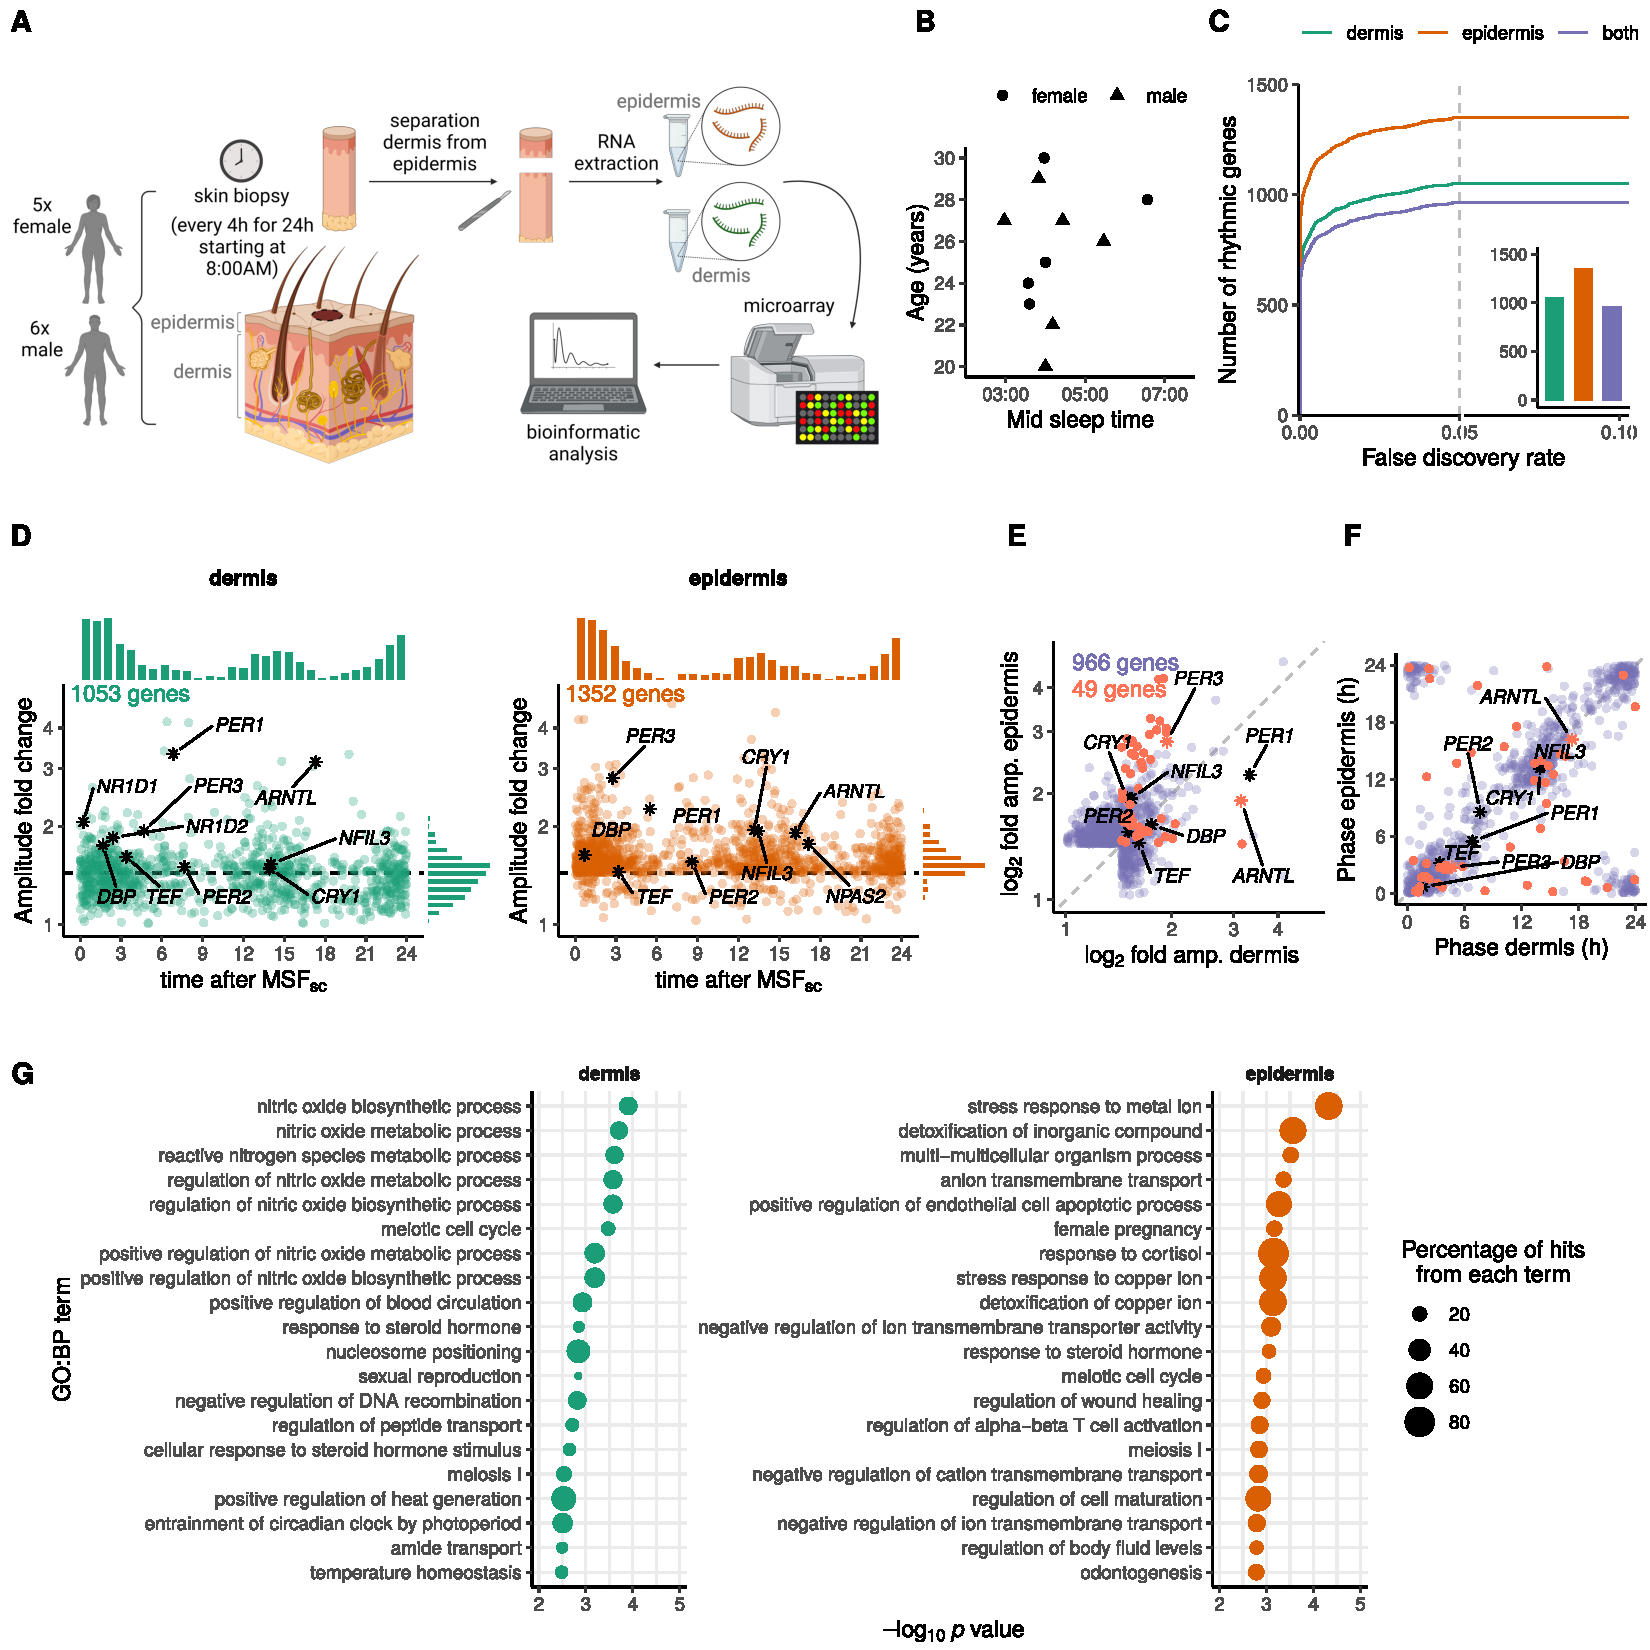
\includegraphics[scale=0.55]{./Figures/fig1_complete.pdf}
		%\caption{\textbf{Functional (and different) clocks in human dermis and epidermis. A.} Experimental setup: the dataset includes dermis and epidermis samples collected from 11 subjects (5 females, 6 males) from the \textcolor{red}{arm}. Skin biopsies were collected every 4\,h for 24\,h starting at 8\,AM. Dermis and epidermis were separated \textcolor{red}{...} and gene expression was analyzed using microarrays.\textbf{ B. }Composition of the study cohort by sex, age and mid sleep time. \textbf{C. }Number of circadian transcripts as a function of the false discovery rate (FDR). Rhythmic transcripts in dermis, epidermis or in both layers were determined by cosinor analysis (\textcolor{red}{FC amplitude$>0.26$}, one single test, in the lines of \cite{Pelikan2021}). Internal time was used for the analysis and was calculated as wall time (i.e., time of sampling) minus the difference in mid sleep time of each subject to a reference subject (that with median mid sleep time). For FDR$=0.05$, 523 transcripts were found to oscillate with a circadian period in dermis, 1191 in epidermis and 283 were common in both layers (bar plots from inset, \textcolor{red}{FC amplitude$>0.26$}). \textbf{D. }Acrophase and amplitude distributions of the 24\,h cycling transcripts in human dermis (in green, left panel) and epidermis (orange, right panel). Each transcript is represented by a dot; clock genes are highlighted in black. Acrophases and amplitudes were estimated from the cosinor analysis at FDR$<0.05$; \textcolor{red}{the minimal FC amplitude for cycling transcripts was set to 0.26}. \textbf{E. }Amplitude correlation of cycling transcripts in dermis \textit{and} epidermis. \textbf{F. }Phase correlation of cycling transcripts in dermis \textit{and} epidermis. \textbf{G.} Circadian GO enrichment analysis of the rhythmic genes in dermis (green) and epidermis (orange). The top 20 enriched biological processes (with a minimum gene set of 5 terms from each category) in each layer are shown. } %Thresholds: transform $\log(1+0.2)$ to ``biological words''.Maybe TODO: use internal time together with amp and phase fits to plot the gene expression curves in all 11 subjects. Then plot mean curve and determine amplitude from the population curve. Do the same but with wall time: Do amplitudes change? For which genes? \textcolor{red}{Think about DOSE with weights -- there was one skin term! Commented at end of 4th paragraph}. mingene set size=5}
%\label{fig:fig1}
	\end{center}
\end{figure*}
\newpage
\begin{figure*}%[htb!]
	\begin{center}
		%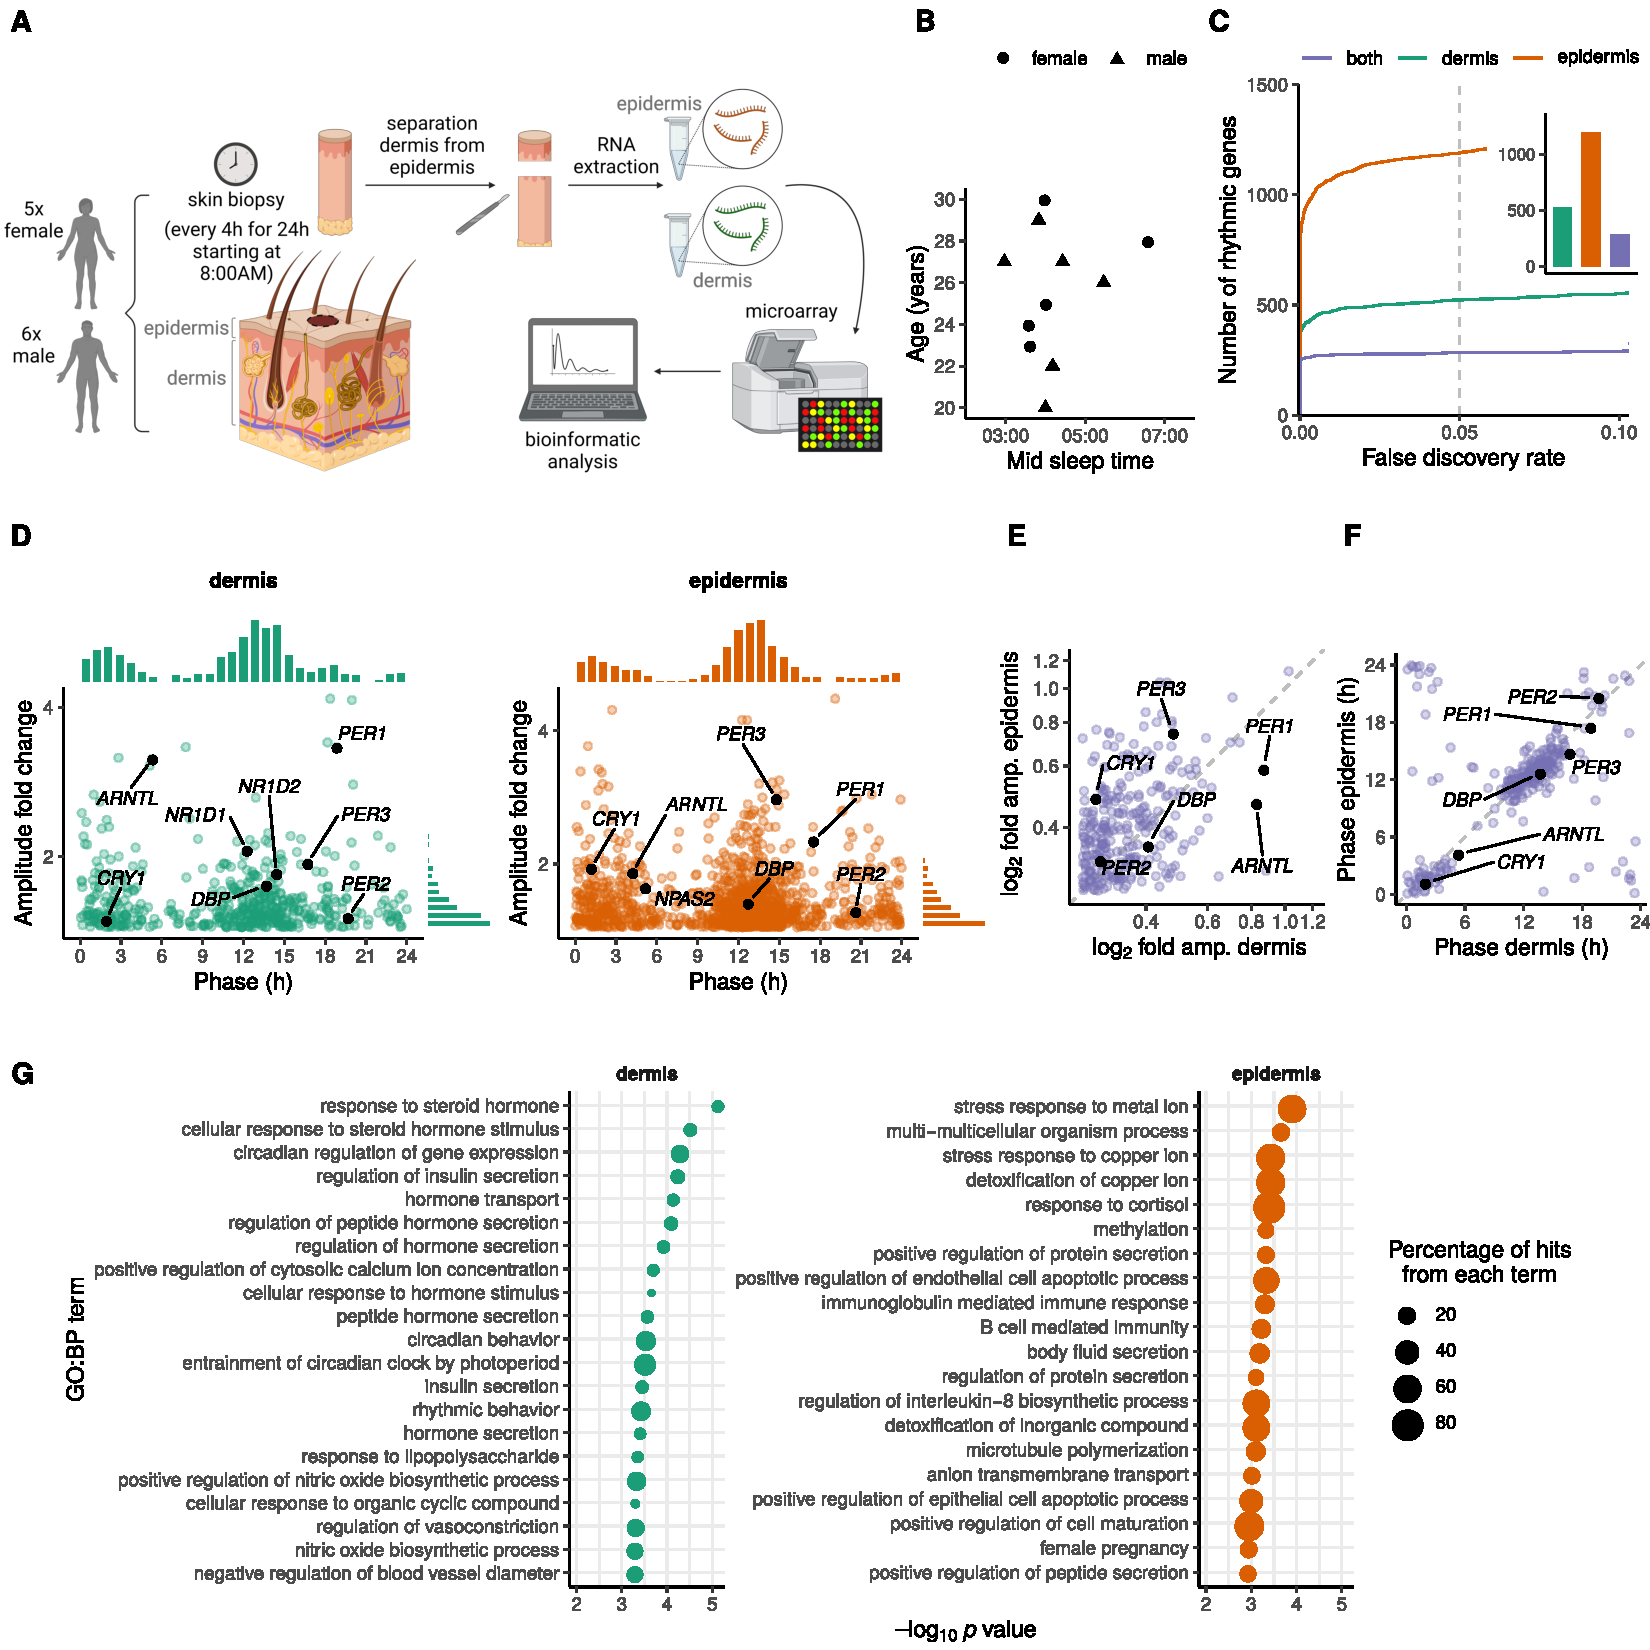
\includegraphics[scale=0.55]{./Figures/fig1_complete_ext.pdf}
		\caption{\textbf{Functional clocks in human dermis and epidermis. A.} Experimental setup: the dataset includes dermal and epidermal samples collected from the back of 11 healthy subjects (5 females, 6 males). Punch biopsies were collected every 4\,h for 24\,h starting at 8\,AM. Dermis and epidermis were separated and gene expression was analyzed using microarrays.\textbf{ B. }Composition of the study cohort by sex, age and mid sleep time. \textbf{C. }Number of circadian transcripts as a function of the false discovery rate (FDR). Rhythmic transcripts with respect to \textit{internal} time in dermis, epidermis or in both layers were determined by cosinor analysis (relative amplitude $>0.26$). For FDR$=0.05$ (inset), 523 transcripts were found to oscillate with a circadian period in dermis, 1191 in epidermis and 283 were common in both layers. \textbf{D. }Acrophase and amplitude distributions of the 24\,h cycling transcripts in human dermis (in green, left panel) and epidermis (orange, right panel) (FDR$<$ 0.05, relative amplitude $>$ 0.26). Each transcript is represented by a dot; clock genes are highlighted in black. \textbf{E. }Amplitude correlation of cycling transcripts in dermis \textit{and} epidermis. \textbf{F. }Phase correlation of cycling transcripts in dermis \textit{and} epidermis. \textbf{G.} Circadian GO enrichment analysis of the rhythmic genes in dermis (green) and epidermis (orange). The top 20 enriched biological processes (with a minimum gene set of 5 terms from each category) in each layer are shown. } %Thresholds: transform $\log(1+0.2)$ to ``biological words''.Maybe TODO: use internal time together with amp and phase fits to plot the gene expression curves in all 11 subjects. Then plot mean curve and determine amplitude from the population curve. Do the same but with wall time: Do amplitudes change? For which genes? \textcolor{red}{Think about DOSE with weights -- there was one skin term! Commented at end of 4th paragraph}. mingene set size=5}
		\label{fig:fig1}
	\end{center}
\end{figure*}

%as many external factors as possible, including chronotype

We observed a bimodal distribution of phases of all circadian dermal and epidermal genes, with peaks clustering at 2\,h and 13\,h after mid-sleep time on free nights (MSF\textsubscript{sc}, Figure \ref{fig:fig1}D and Supplementary Figure \ref{fig:suppfig2}A)\todo{in contrast to previous studies that have reported phases clustered at 8:00-9:00 and 20:00-21:00 \cite{Wu2018, Wu2020}).}. Despite the similarity of the distributions, amplitudes and phases of individual genes varied between skin layers: Among rhythmic genes common to the two layers, \todo{consistently use circadian genes or genes with circadian expression} epidermal circadian genes oscillate with a higher amplitude than those in the dermis among the differentially-rhythmic genes, with a trend in this direction among the circadian genes with similar rhythms (Figure \ref{fig:fig1}E). There was no systematic trend in the phase difference between common circadian genes in the two layers (Figure \ref{fig:fig1}F). The core clock genes were remarkably consistent (statistically indistinguishable) in amplitude and phase between the two layers (Supplementary Figure \ref{fig:suppfig2}B) with the exception of \textit{ARNTL} and \textit{PER3}, which had higher amplitudes in the dermis and epidermis, respectively. Note, NR1D1 and NR1D2 were rhythmic in both layers but with amplitudes just outside the amplitude cutoff in the epidermis.

Dermal circadian genes were enriched in nitric-oxide metabolism, photoperiodic response, hormone-related terms and blood circulation, whereas the epidermis circadian transcriptome was enriched in terms related to the response to metals, regulation of fluid levels and wound healing, and response to cortisol (Figure \ref{fig:fig1}G). We also performed KEGG pathway enrichment analysis and found that infection-related and TNF signaling pathways appeared in dermis; on the other hand, the epidermal circadian genes was enriched in pathways associated to metabolism and phototransduction (Supplementary Figure \ref{fig:suppfig2}C). Morning-time genes were enriched for immune-related pathways together with phosphorylation and metabolic signaling, whereas the evening was marked by genes involved in carbohydrate, nitrogen and phenol metabolism (Supplementary Figure \ref{fig:suppfig2}D and E, as determined by phase set enrichment analysis (PSEA) \cite{Zhang2016}). \todo{is this phase, time after MSFsc?}

Interestingly, the circadian genes determined with respect to external time (Supplementary Figure \ref{fig:suppfig1}) did not deviate appreciably in number, amplitude or phase from the circadian genes (Figure \ref{fig:fig1}C,D,E,F) with respect to internal time, i.e, controlling for $\textrm{MSF}_\textrm{sc}$ did not affect rhythmicity analysis significantly in our dataset. \todo{for discussion -- This might be due to the range of MST, which is in the order of the sampling frequency, or because of additional sources of inter-individual variation.} In summary, we observed significant similarity in the circadian gene expression across these two adjacent skin layers complemented by some layer-specificity of circadian rhythms. 

%\textcolor{red}{\textbf{I've removed the correlation matrices from this figure}}.\\%To our surprise, we found no skin-related diseases when doing disease ontology enrichment analysis \cite{Yu2015}, but several pancreatic and cardiovascular-related conditions enriched in dermis (no significant diseases were enriched among the circadian epidermal transcriptome) (Figure \ref{fig:fig1}H).\\

%\scriptsize{\textcolor{red}{Are the most rhythmic genes in each layer related to a specific function? e.g. keratinization in epidermis? Also2: Do phases of genes correlate with the mid sleep time? I guess this question applies mostly to phases of ZeitZeiger genes}.}

%\footnotesize{\begin{itemize}
%	\item Human dermis and epidermis every 4h across a 24-h sampling period from 11 individuals (starting at 8\,AM)
%	\item \textbf{\underline{One}} single test (in the lines of \cite{Pelikan2021}) to identify rhythmic genes only in dermis versus only in epidermis versus in both layers.
%	\item Stable number of rhythmic genes independently of the exact FDR cutoff
%	\item Wall time corrected with mid sleep time $\rightarrow$ internal time: we think internal time should be taken into account if any evaluation of circadian phase of skin biomarkers is desired.
%		\begin{itemize}
%		\item Wall time and internal time give similar numbers of rhythmic genes $\rightarrow$ maybe because mid sleep time range is $\sim$ our sampling frequency?
%	\end{itemize}
%	\item Functional clocks present in human dermis and epidermis
%	\begin{itemize}
%		\item Careful with conclusions about tissues -- skin is very heterogeneous with various tissue types 
%		\item Clock amplitude and phase varies between skin layers: higher amplitude in epidermis (reason for more rhythmic genes?), dermis is later
%	\end{itemize}
%	\item Identification of clock-regulated transcriptome in human skin layers: we compared the circadian transcriptome of the two prominent skin layers in human skin, i.e. dermis and epidermis
%	\begin{itemize}
%		\item Amplitude and phases vary in similar fashion as do the clock genes
%		\item Bimodal phase distribution: two main peaks ast $\sim1$\,AM and $\sim1$\,PM \textcolor{red}{($\neq$Hogenesch!)}
%	\end{itemize}
%	\item GO terms (\textcolor{red}{KEGG better?}) all over the place \textbf{\textcolor{red}{-- slim them!}}, and not super significant:
%	\begin{itemize}
%		\item Dermis: rhythmic processes, hormone-related terms, blood vessel related processes \textcolor{red}{(viral, parasite and bacteria-related pathways)}
%		\item Epidermis: response to metals, immune-related terms, body fluid and protein secretion \textcolor{red}{(absorption, phototransduction, immune-related pathways)}
%	\end{itemize}	
%	\item Disease enrichment: related to cardiovascular disease, pancreatic conditions
%	\begin{itemize}
%		\item No skin-related conditions like psoriasis for example \textcolor{red}{-- move to the supplement?}
%	\end{itemize}	
%	\item \textcolor{red}{Are the most rhythmic genes in each tissue related to a specific function? e.g. keratinization in epidermis?}
%\end{itemize}}

%----------------------------------------------------------------------------------------
%----------------------------------------------------------------------------------------

\subsection*{Variation in circadian gene expression in the skin}
The population (mean) circadian gene expression represents rhythmic gene expression at the level of the cohort. We next evaluated how variable circadian expression was within the cohort in relation to the variability across layers. In other words, how representative is the population gene expression of circadian expression in individuals. We fit linear-mixed-effect models \cite{Hoffman2016} followed by error propagation to obtain both the average circadian gene expression (fixed effects) and the variation across subjects and layer (random effects). For this analysis, we only considered the 1439 genes that showed rhythms at the population level in at least one layer. We characterized the variability in circadian parameters (magnitude (MESOR), amplitude and phase) of individual rhythmic genes across layers and subjects.

Magnitudes varied more across layers, and amplitudes and phases more across subjects. The error propagation analysis produced estimates of the variances of the circadian parameters across subjects and layers. We simultaneously characterized this variability in relation to the population circadian parameters using the coefficient of variation (CV). When the variability is viewed in absolute or relative terms, magnitude of circadian genes varied more across layers than across subjects, while amplitudes and phases were more variable across subjects than across layers (Figure \ref{fig:fig2}A). In order to better quantify the relative contribution of layer and subject to the circadian rhythm variability, we defined the fraction of variance explained by subject as $\sigma^2_\textrm{sub}/(\sigma^2_\textrm{sub} + \sigma^2_\textrm{lay})$ \todo{plot vs CV in supplement.}

Amplitudes of rhythmic genes were more variable than phases. The percentage variation of amplitude exceeded variation of phases both across layers and across subjects (Figure \ref{fig:fig2}C). Genes with different population rhythms between layers (Figure \ref{fig:fig1}) showed high amplitude and phase variability across layers as expected In agreement with population rhythm analysis, core clock genes had remarkably low variability in amplitude and phases across layers. However, the core clock genes were more phase variable across subjects, but with comparable amplitude variability across subjects and layers. \todo{is there more to unpack here? I cant see the grey points much at all.}






%The total expression variance of a gene can be partitioned into the individual contributions of subject, sex, skin layer and time plus a residual variance. This simple model assumes that the effect of each component of variation on the gene expression is additive and independent of other components in the model. To relax this strict assumption, we also modeled interaction effects whereby the effect of time depended also on subject and skin layer. In the end, we quantified six sources of variability: 
%\begin{itemize}
%	\item inter-sex mean variation (variance in mean expression (magnitude) between males and females),
%	\item inter-layer mean variation (variance in magnitude only due to differences in skin layers),
%	\item inter-subject mean variation (variance in magnitude only due to differences between subjects), 
%	\item common circadian variation (variation in expression across time points common to all layers and subjects), 
%	\item inter-layer circadian variation (variance of the temporal profiles across the two layers) and
%	\item inter-subject circadian variation (variance of the temporal profiles across subjects).
%\end{itemize}
%With the number of subjects and samples per subject in this study, other two-way and multi-way interactions could not be determined using this data. 

\begin{figure*}[b!]
	\begin{center}
		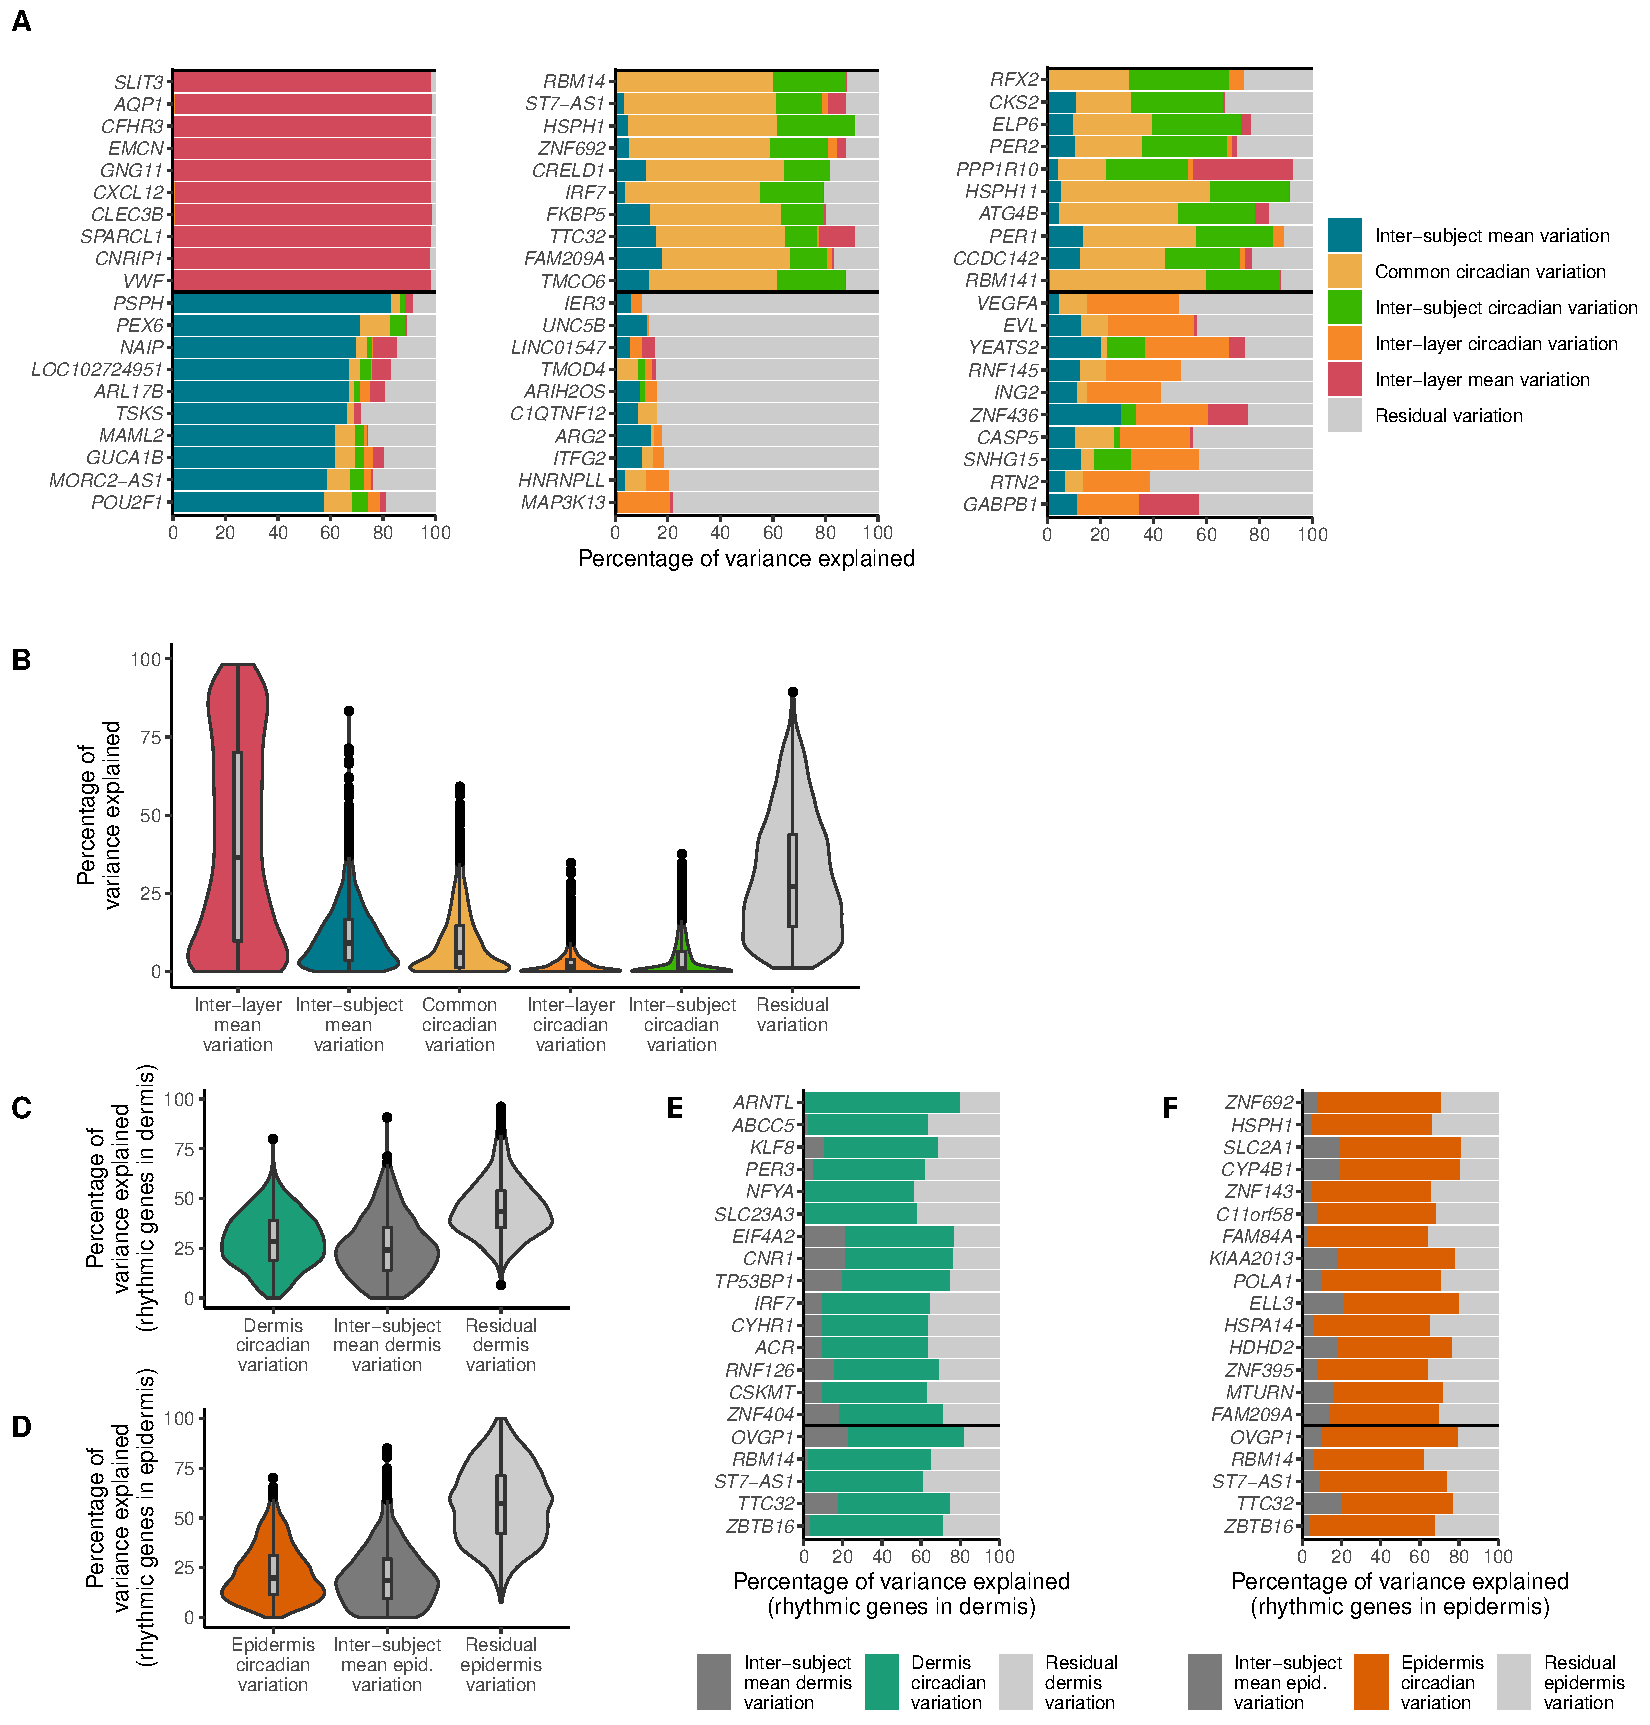
\includegraphics[width=\textwidth]{./Figures/fig2.pdf}
		%\caption{Identification of drivers of variation from the circadian transcriptome in human skin with variancePartition \cite{Hoffman2016}. A. Top 10 genes with highest variance in mean expression across layers (top left panel), across subjects (bottom left panel), across time (top middle panel) or with highest residual (unidentified) variation. The panels in the right show the top 10 genes with highest differences in circadian expression across subjects (i.e., rhythmic transcripts where rhythms seem to be subject-specific, top panel) or with highest differences in circadian expression across skin layers (i.e., rhythmic transcripts where rhythms seem to be dermis- or epidermis-specific, bottom panel). \textcolor{red}{Note how these results illustrate how variancePartition identifies genes where the majority of variation in mean expression is explained by a single variable, such as skin layer for \textit{SLIT3}, while variation in other genes is driven by multiple variables \textit{ZNF436}}. B. Quantification of the contribution of each meta-data variable to the variation in expression of each gene in a circadian transcriptome-wide trend, with the total contribution of each variable ranked in order from left to right (except the residual variation). \textcolor{red}{Should I make clear here what each metavariable means?}. To plot panels A and B, variancePartition was run with the $\sim~1400$ genes that are rhythmic in \textit{at least} one tissue and with external time as a meta-data variable (since internal time, a continuous variable, cannot be modeled as a random variable).}
		
		% \textcolor{red}{We previously argued that the common circadian variation is larger than the inter-subject/inter-layer circadian variation, and that this could be a reason to do ZeitZeiger on the whole dataset and not in dermis versus epidermis. If we are going to do ZeitZeiger on the whole dataset, should we maybe move panels C-F to the Supplement? They are still `informative' in the sense that they show that, taking all rhythmic genes in dermis (or epidermis), the largest source of variation in mean expression is variability across time and not subjects.}}
		%\label{fig:fig2}
	\end{center}
\end{figure*}

\begin{figure*}[!]
	\begin{center}
		%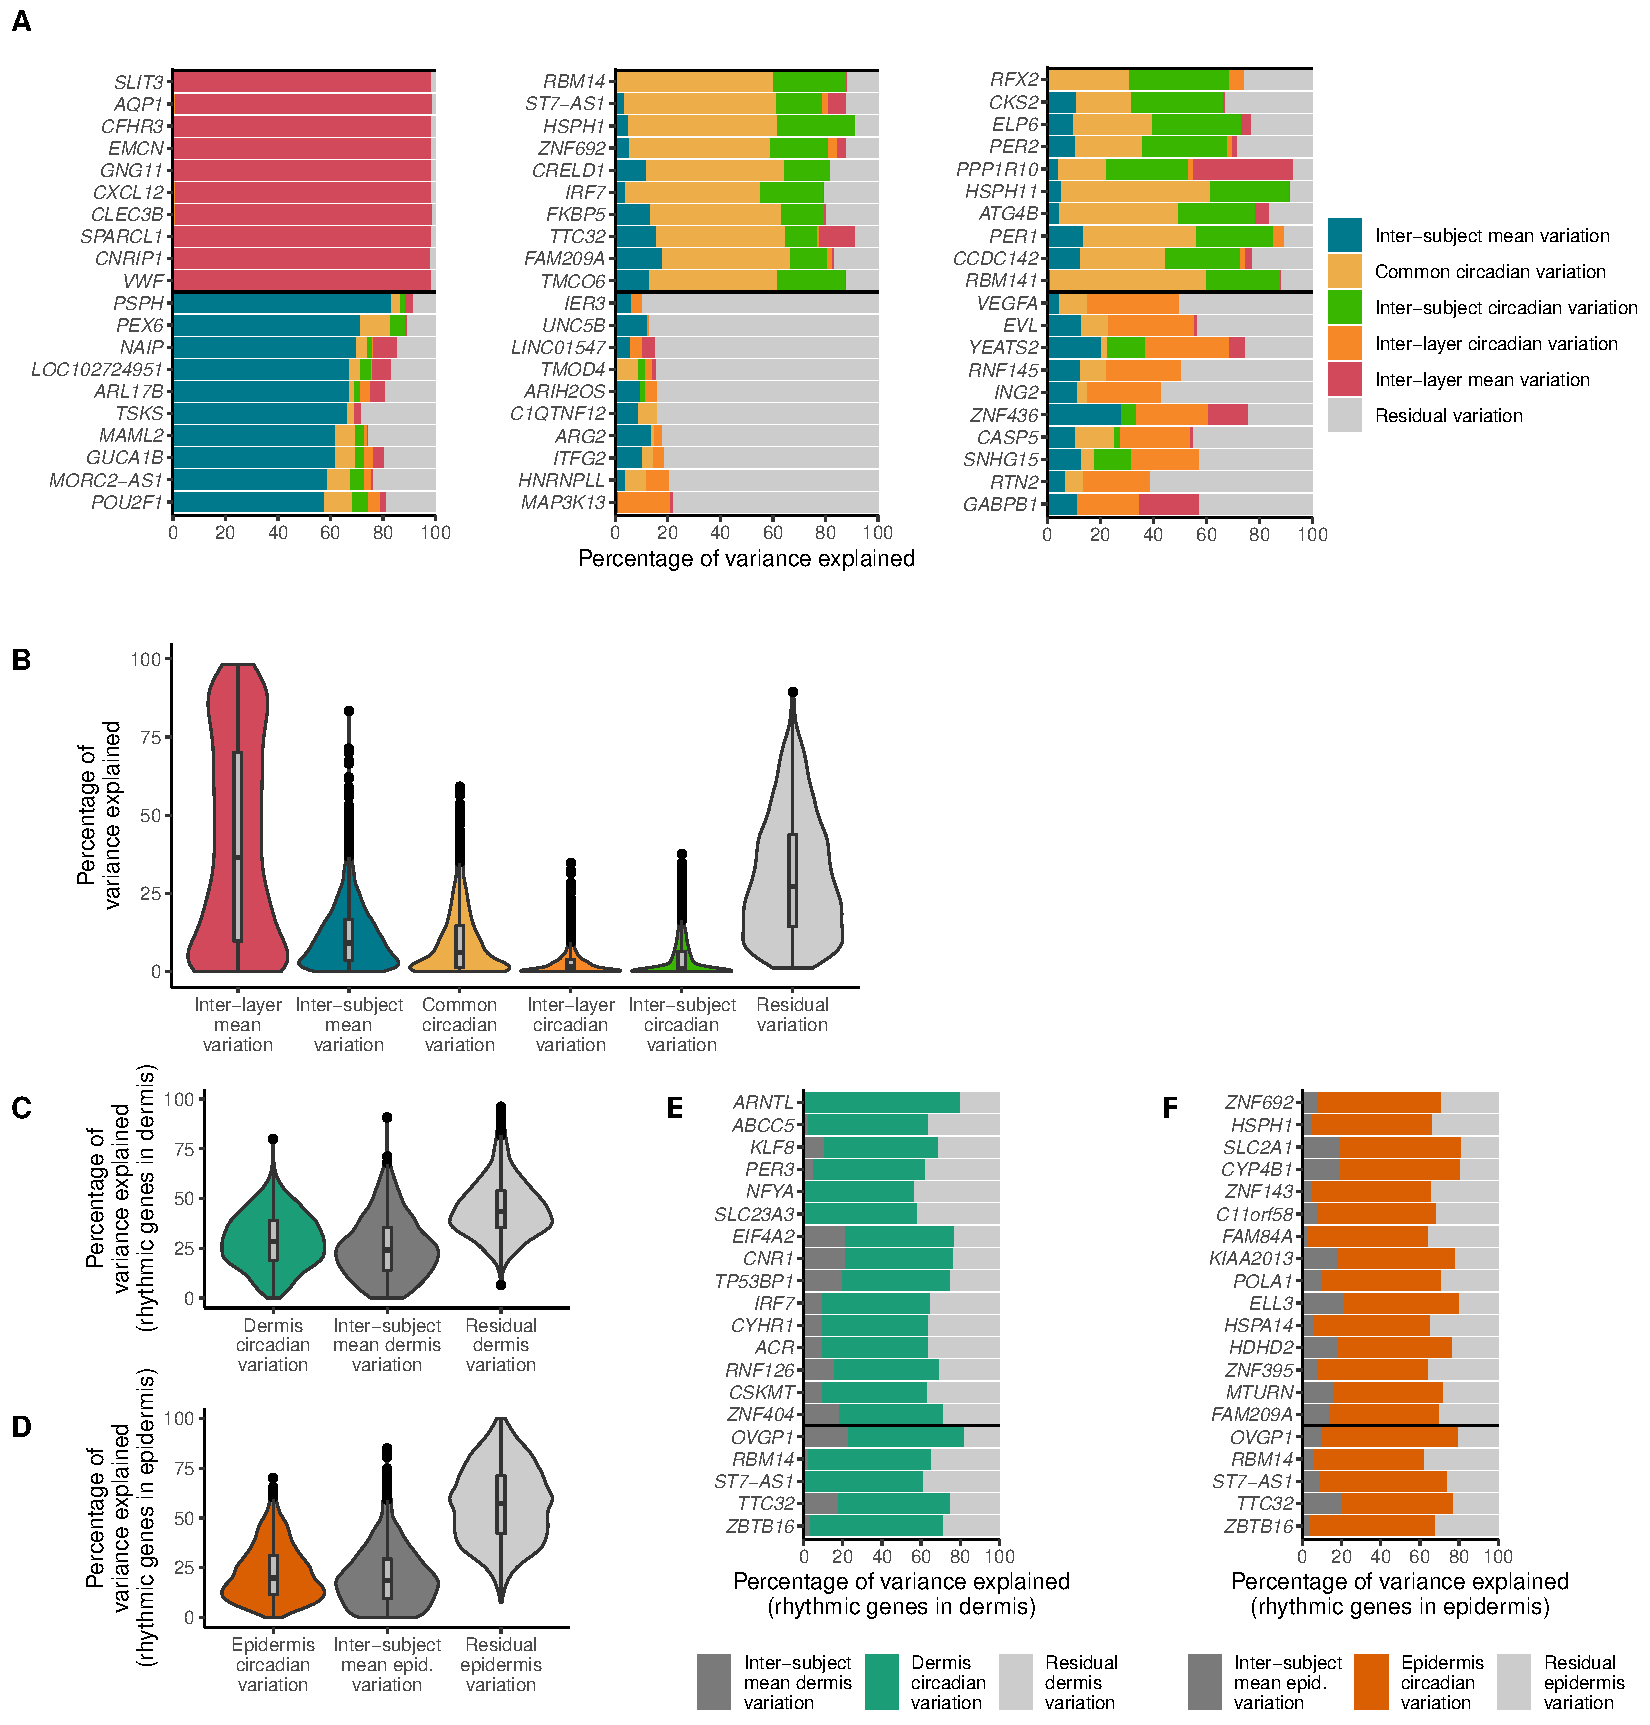
\includegraphics[scale=0.55]{./Figures/fig2.pdf}
		\caption{\textbf{Drivers of variation in the human circadian skin transcriptome identified with variancePartition. A.} Top 10 genes with highest variance in mean expression across layers (top left panel), across subjects (bottom left panel), across time (top middle panel) or with highest residual (unidentified) variation (bottom middle panel). The panels in the right show the top 10 genes with highest differences in circadian expression across subjects (i.e., rhythmic transcripts where rhythms seem to be subject-specific, top panel) or with highest differences in circadian expression across skin layers (i.e., rhythmic transcripts where rhythms seem to be layer-specific, bottom panel). \textbf{B.} Quantification of the contribution of each meta-data variable to the variation in expression of each gene in a circadian transcriptome-wide trend. To plot panels A and B, variancePartition was run with the $\sim1400$ genes that are rhythmic in \textit{at least} one layer and with external time as a meta-data variable. \textbf{C} and \textbf{D.} Contribution of each variable to variation in mean expression in the rhythmic genes in dermis (C) and epidermis (D). \textbf{E} and \textbf{F. } 20 genes with highest variation across time in dermis (E) and epidermis (F). Common time-varying genes across layers are depicted below the black line in panels E and F. variancePartition was run with the 523 rhythmic genes in dermis to plot panels C and E and with the 1191 rhythmic genes in epidermis to plot panels D and F.}
		
		% \textcolor{red}{We previously argued that the common circadian variation is larger than the inter-subject/inter-layer circadian variation, and that this could be a reason to do ZeitZeiger on the whole dataset and not in dermis versus epidermis. If we are going to do ZeitZeiger on the whole dataset, should we maybe move panels C-F to the Supplement? They are still `informative' in the sense that they show that, taking all rhythmic genes in dermis (or epidermis), the largest source of variation in mean expression is variability across time and not subjects.}}
		\label{fig:fig2}
	\end{center}
\end{figure*}
%Applying variancePartition to this data illustrates how the method can decouple biological variation into multiple components, including a residual variation which remains uncharacterized. Results from representative genes \todo{I think I like looking at the transcriptome wide result before we look at individual genes. Although I get what you are trying to do here.}show how variancePartition identifies genes where the majority of variation in mean expression is explained by a single variable such as skin layer (e.g., \textit{SLIT3}, Figure \ref{fig:fig2}A, left panel), while variation in other genes is driven by multiple variables (e.g. \textit{ZNF436}, Figure \ref{fig:fig2}A, right panel). These results, illustrated in a rhythmic skin transcriptome-wide manner, show that variation across skin layers represents the major source of magnitude variability and explains a median of 36.4\% of the variance from the rhythmic skin transcriptome (Figure \ref{fig:fig2}B). The median variance explained \todo{I dont think absolute values of the variance explained mean much with interaction terms, see variancePartition} by subject (9.1\%), common circadian variation (6.1\%), inter-layer circadian variation (1.4\%) and inter-subject circadian variation (0.9\%) are smaller, but with a high unidentified residual variation (27.3\%). Moreover, we found that neither chronotype nor sex contribute to variability in mean expression of rhythmic genes, as \texttt{variancePartition} attributed very little variance to these components ($<0.5$\%, \textcolor{red}{data not shown}). \\

%Of particular interest here were two things: firstly, the fact that subjects differ more strongly in mean expression than in circadian rhythms (compare blue violin plot to green violin plot from Figure \ref{fig:fig2}B). This means that although rhythms \textcolor{red}{(phases?)} of clock controlled genes are not very subject-dependent, their magnitudes are. Secondly, the observation that time variation does not seem to be layer- or subject-specific, since the inter-subject and inter-layer circadian variation appeared smaller than the common circadian variability. In other words, time alone can explain variation without being dependent on layer or subject in our cohort. This result, together with the almost nonexistent contribution of chronotype to variability and the findings from Supplementary Figure \ref{fig:suppfig1}, speaks for population sampling from skin providing a good estimation of circadian time, regardless of wall time or internal time. As negative and positive control of the variancePartition analyses, we checked that the time variation across 1000 non-rhythmic genes (FDR $>0.1$) was almost 0 (Supplementary Figure \ref{fig:suppfig3}A), while it represented the largest source of variation for clock genes (Supplementary Figure \ref{fig:suppfig3}B).\\ %Interestingly, we also found the residual variation to be high in previous human skin transcriptomic datasets \cite{GSE112660, GSE139300} that we reanalyzed (\textcolor{red}{data not shown}). 
%BA1: common circadian variation is strongest in our cohort so we expect these insights to translate across population.
%BA2: great that subject differs in mean a lot but not so much in circadian - I think it is not obvious/known that CCGs' magnitude varies quite a lot between subjects.

%\textcolor{red}{We performed \textcolor{red}{GO analysis in top 200 most variable genes from each category} and found that wound healing processes were enriched in those with high variation in mean expression across layers (\textcolor{red}{Supplementary Figure \ref{fig:suppfig3}C}). On the other hand, genes with highest circadian variation across skin layers (orange category from Figure \ref{fig:fig2}A) were enriched in pyruvate metabolism, phosphorylation and ATP generation processes (Supplementary Figure \ref{fig:suppfig3}D). As for the genes with highest (unidentified) residual variation, we found that they were enriched in processes related to cytoskeleton and stimuli detection (\textcolor{red}{Supplementary Figure \ref{fig:suppfig3}E}).\\}

%Performing \texttt{variancePartition} on the epidermal and dermal rhythmic genes separately hinted to what the drivers of variation in each layer separately are. Common circadian variation exceeded the inter-subject mean variation in gene expression in both skin layers (although the residual variation, in either case, was found to be larger than the other sources of variation, Figure \ref{fig:fig2}C, D). The clock genes \textit{ARNTL, PER3} were found among the top 20 common circadian varying genes in dermis, but not in epidermis (Figure \ref{fig:fig2}E). Some genes appeared to have a high variability across time in both layers: \textit{OVGP1, RBM13, TTC32} or \textit{ZBTB16} (shown in the bottom of Figure \ref{fig:fig2}E, below the black line). \\

%Of note, the variance in mean expression explained by skin layers represents also the highest source of variation in previously published skin circadian transcriptomic studies \cite{GSE112660, GSE139300}, and these also show high residual variability (\textcolor{red}{data not shown}). This suggests that the learnings from our dataset can be translated to larger populations. Interestingly, the quantification of variation in our data is robust to sampling frequency. This is, we found similar contributions of each biological source when the time series of rhythmic genes was made sparser by removing time points (\textcolor{red}{data not shown}). \\%\\
%\footnotesize{\begin{itemize}
	%\item We quantified inter-subject and inter-layer variability in mean and circadian expression of clock-controlled genes -- explain these these categories (e.g. genes with high ``inter-layer circadian variation'' refers to those genes that show different circadian rhythms between both layers, and genes with high ``inter-subject circadian variation'' refers to those rhythmic genes that vary between subjects)
%	\item Common circadian variation exceeds inter-subject and inter-layer circadian variation, thus we expect to find good time-telling genes sets even across layers \textcolor{red}{$\rightarrow$ reason to do ZeitZeiger on the whole dataset and not in dermis versus epidermis?}
	%\begin{itemize}
		%\item Inter-layer variation represents the biggest source of variability in mean expression. It is followed by mean inter-subject variation, which in turn exceeds common circadian variation. 
		%\item Big residual variation 
	%\end{itemize}	
	%\item Also Hogenesch's data shows big residual variation
	%\item Chronotype doesn't matter in skin: population sampling from skin provides a good estimation of circadian time (regardless of wall time or internal time)
	%\item Results independent of the number of datapoints taken (with 4 data points, similar variances -- data not shown)
%\end{itemize}}

%----------------------------------------------------------------------------------------
%----------------------------------------------------------------------------------------

\subsection*{Predictive biomarkers of internal time in human dermis and epidermis}
As the most exterior human organ, the skin provides a good source of circadian biomarkers. When we assume that the skin clock maintains fixed phase relationship with the central clock in the SCN, these markers can serve as predictors of circadian phase of entrainment or chronotype. We identified biomarkers to predict \textit{internal} time using \texttt{Zeitzeiger} from genes expressed in either layer individually and in both layers together.

%Details on the ZeitZeiger implementation and the main parameters it uses are provided in Materials and Methods. \\
The layer specificity of circadian gene expression in the skin that we observed compels a search for biomarkers in each layer individually. For an optimal choice of parameters (2 sparse principal components (SPC) and sparsity ($sumabsv$)=2)), 15-25 rhythmic genes were sufficient to predict internal time with a median absolute error (MAE) of $\sim 0.96$\,h (Figure \ref{fig:fig3}A). In both layers, a high proportion of the time-telling genes overlapped with the top 20 time-varying genes from VPA (highlighted in yellow in Figure\ref{fig:fig3}B). (\textit{OVGP1} was not only a highly time-varying gene, but also one of the top 20 genes that have different rhythms in epidermis compared to dermis (orange category from Figure \ref{fig:fig2}), and hence marked orange). In fact, on repeating VPA only on circadian biomarker genes, we found that common circadian variance represented the dominant driver of expression variation in both skin layers, while inter-subject variation  was minimal (\todo{does not match Supplementary Figure \ref{fig:suppfig5}B, also evident from the time series in Supplementary Figure \ref{fig:suppfig5}A}). In other words, biomarkers of circadian phase show little differences in mean expression (i.e., magnitude) across subjects and also possess strong circadian rhythms. 

Interestingly, the projection of dermal and epidermal samples on to the SPCs described a cycle for which the progression of internal time followed a counter-clockwise trajectory in both skin layers (Figure \ref{fig:fig3}C). These results imply that the circadian clock is well approximated by a two-dimensional oscillator. Moreover, this cyclical behavior in SPC space was observed for each individual subject (Supplementary Figure \ref{fig:suppfig5}C), \todo{ better in Discussion? suggesting that such an approach may be used to detect perturbations of the skin clock in humans}. \\



\begin{figure*}[t!]
	\begin{center}
		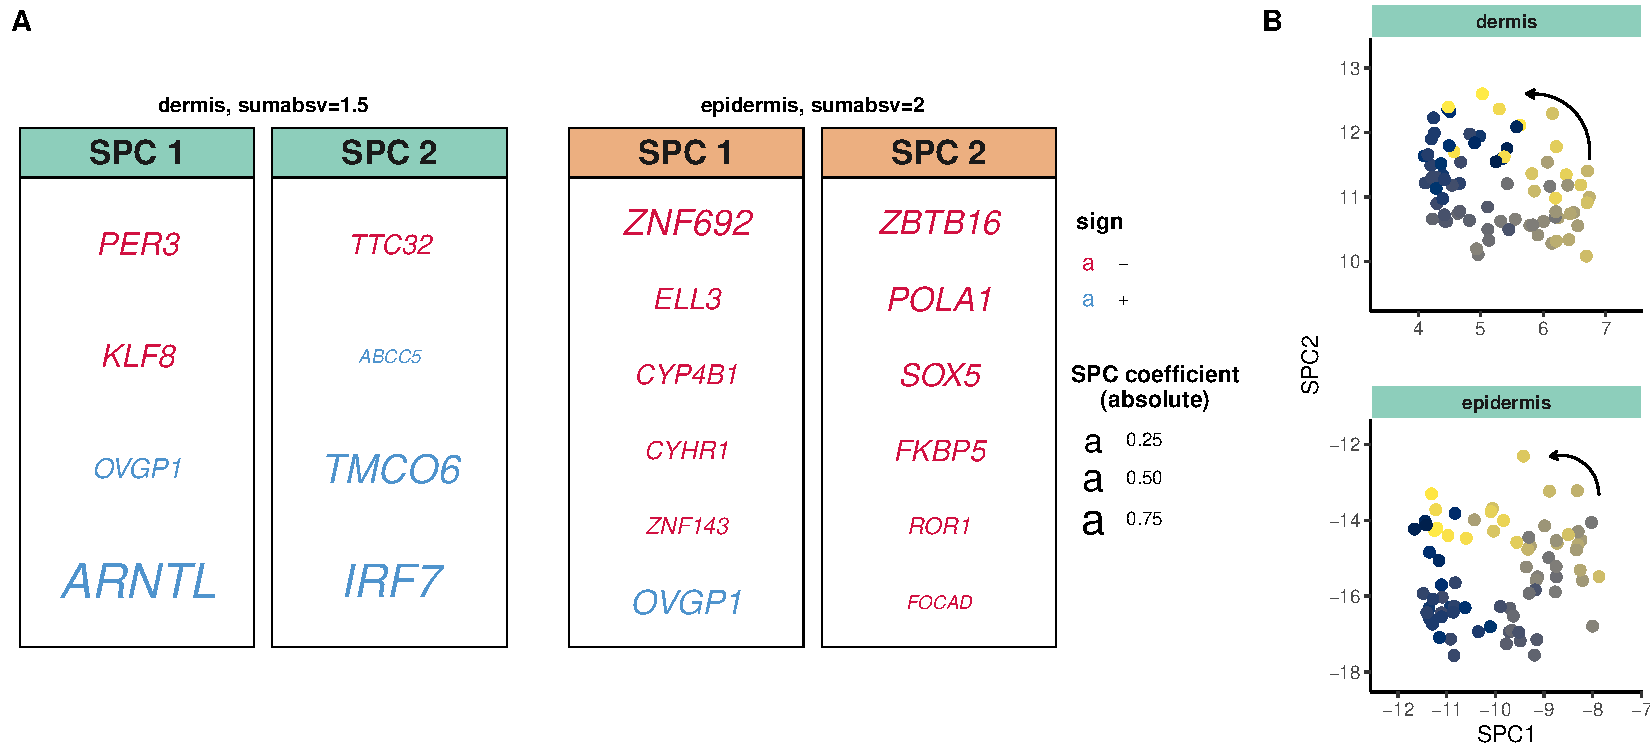
\includegraphics[scale=0.55]{./Figures/fig3.pdf}
		\caption{\textbf{Identification of internal time-telling genes in human dermis and epidermis with \texttt{ZeitZeiger}. A. }Median absolute error of the internal-time prediction on cross-validation (see Materials and Methods for details) as a function of the two main parameters of ZeitZeiger, \texttt{sumabsv} and \texttt{nSPC}. \textbf{B. }Internal time predictors from human dermis (left panels) and epidermis (right panels) for \texttt{sumabsv}=2 and \texttt{nSPC}=2. Genes assigned to SPC1 or SPC2 as well as their coefficients are shown. Highlighted in yellow are genes that appeared in the top 20 most common circadian varying genes in the variancePartition analysis done in dermis and epidermis separately; in orange, genes that showed differential rhythms across layers (i.e., genes with high inter-layer circadian variation from the variancePartition analysis). \textbf{C. }Expression profiles of our cohort in dermis (left) and epidermis (right) represented in SPC space. Colors indicate the internal time of the subjects. ZeitZeiger was run with all $\sim11000$ expressed genes and separately for dermis and epidermis.}
		\label{fig:fig3}
	\end{center}
\end{figure*}

%To measure the accuracy of the prediction, \texttt{ZeitZeiger} uses the median absolute error (MAE): the lower this value, the better the prediction. Running \texttt{ZeitZeiger} in the whole set of $\sim11000$ skin-expressed genes (in either dermis \textit{or} epidermis) resulted in a minimum MAE of $\sim0.08$ for the software parameters \texttt{nSPC}=2 and \texttt{sumabsv}=3 (Supplementary Figure \ref{fig:suppfig4}A), with 38 genes needed for prediction (Supplementary Figure \ref{fig:suppfig4}B). On the other hand, running \texttt{ZeitZeiger} in each skin layer separately performed better, as seen by the lower MAE and the lower number of genes needed to predict internal time: 2 SPCs and \texttt{sumabsv}=2 resulted in a MAE of 0.04 in both layers (Figure \ref{fig:fig3}A) and a total of 15-25 genes needed for prediction (Figure \ref{fig:fig3}B, time series in Supplementary Figure \ref{fig:suppfig5}).\\ %\textcolor{red}{All three/two?} predictors performed comparably well, since the MAE did not decrease much after 2 sparse principal components (SPCs). However, the optimal value of \texttt{sumabsv} and, consequently, the number of genes used for prediction, differed in each approach. 

Our results indicate that dermis and epidermis time series data are well suited to extract time-telling genes, and that internal cross-validation performance is similar to that of previous studies \cite{Wu2018, Wu2020} \textcolor{red}{(I'm not sure if sfig7 and sfig8 really support this...)}. Moreover, integrated with prior published circadian skin transcriptomic studies, these results provide robustness, as some of the biomarker genes that we have found have already been described as skin phase-telling genes (\textit{ZBTB16, FKBP5, TRIM35, PER3, ARNTL}) \cite{Wu2018, Wu2020}. Moreover, although the common circadian variability exceeds the inter-subject and inter-layer circadian variation (Figure \ref{fig:fig2}A), and thus one could expect to find good time-telling gene sets even across layers, our results show that predicting internal phase in dermis and epidermis separately performs better than predicting internal time in skin as a whole. \\

\textcolor{red}{Of note, ZeitZeiger was also used to predict external (wall) time. Although the accuracy of wall time predictors was comparable to those of internal time, the value of \texttt{sumabsv} was higher, thus resulting in a larger number of genes needed to predict wall time in both, skin as a whole, and in dermis versus epidermis separately (data not shown).}\\

%\footnotesize{\begin{itemize}
	%\item Zeitzeiger genes don't vary much in mean across subjects (useful) (data not shown)
	%\item ZeitZeiger genes in epidermis also found in Wu2018 \cite{Wu2018}: \textit{ZBTB16, FKBP5, TRIM35}
	%\item ZeitZeiger genes in dermis also found in Wu2020 \cite{Wu2020}: \textit{ZBTB16, PER3, ARNTL}
	%\item Is there a ``better'' marker for skin phase?
	%\item How good are the monocyte biomarkers in skin?
	%\item \textcolor{blue}{ZeitZeiger predicts phase... but can we come up with an amplitude predictor? Ratios of clock genes maybe?}
	%\item More time-telling genes if we use wall time, but since we want to predict \underline{internal} time it maybe makes more sense to use internal time
	%\item Candidate biomarkers that are robust to a different sample collection method?
	%\item Zeitzeiger genes are not any of the top 20 varying tissue-genes (vp full)
%\end{itemize}}




%------------------------------------------------

\section{Discussion}\normalsize
%\textcolor{red}{I think I shold discuss more the different biomarker time-telling approaches that have been imlemented and in which tissues so far -- in the intro I don't have time/space for this: Dijk blood biomarkers, Ueda pioneer... Also sex not contributing}\\

%%Discuss figure 1
We report here a study of circadian gene expression in the skin of 11 \textit{healthy} human subjects sampled longitudinally every 4\,h over a 24\,h period. Unlike previous genome-wide analyses of the human skin \cite{Wu2018,Wu2020}, this dataset contains samples at higher temporal resolution with chronobiological profiles of all study subjects. This latter information allowed us to assess the chronotypes of subjects (as mid-sleep time on free days corrected for sleep debt) and thereby perform all analyses with respect to internal time. The diversity of chronotypes or phases of entrainment in the human population \cite{Roenneberg2007} necessitates such an approach. In other words, molecular rhythms across subjects are expected to be coherent only after chronotype differences are corrected for. Nevertheless, most studies continue to assess population rhythms with respect to wall time (or sample collection times) \cite{Laing2019}. We attempted to quantify the difference in our results between the use of internal and wall times, but the 4\,h sampling resolution is still insufficient to accurately reflect the $\sim$6h range of 95\% of human chronotypes.

The cellular complexity and heterogeneity of human skin suggested that the notion of a singular ``skin clock'' is too simplistic. We therefore determined circadian gene expression in two important skin layers, the dermis and epidermis, in all subjects. We presented a hierarchical description of circadian rhythms in the two layers. First, the population gene expression rhythms represent average rhythms across the cohort. Conceptually, the population rhythms are an estimate of the average rhythms of a hypothetical population of individuals, from which the cohort is randomly sampled. Second, we quantified the variability of circadian rhythms across the cohort as a representation of variability within the hypothetical population.

Our analysis revealed $\sim$1400 circadian genes in either layer at the population level, significantly expanding on the list of known clock output genes in human skin \cite{Wu2018, Wu2020}. However, two-thirds of these genes had indistinguishable rhythms between the layers. On the one hand, this is unsurprising given the physical proximity between the layers. On the other, it is unexpected given the well-documented skin heterogeneity and tissue-specificity of circadian programs in physiology \cite{Ruben2018}. As reported in many studies, the core clock gene expression was consistent between the layers with the exception of \textit{ARNTL} and \textit{PER3}. Despite this general similarity, a third of the circadian genes did display expression in only one or the other layer. On the whole, the epidermal circadian genes tended to have higher amplitudes than the dermal circadian genes (as suggested previously \cite{Wu2020}), which is also reflected in greater number of circadian genes in the epidermis compared to the dermis. We can only speculate that this might be because of the direct environmental exposure of the epidermis to external Zeitgebers.


%Here we report a novel human dataset in which we examined circadian gene expression of skin in 11 subjects that were sampled longitudinally every 4\,h for 24\,h. Although skin circadian rhythms have been analyzed in previous studies in a genome-wide manner \cite{Wu2018, Wu2020}, this dataset has a higher sampling frequency and contains information about the subjects, what allows to control for external factors and to assess what the sources of variation in such a human study might be. We identified the circadian transcriptome of human dermis and epidermis with respect to \textit{internal} time by correcting external time to each individual's mid sleep time. We found that roughly a fifth of the circadian skin transcriptome ($\sim$280 out of 1400 rhythmic genes) is shared between both layers, while a large part is layer-specific. Interestingly, and despite their physical proximity, we found amplitude and phase differences in the core clock and clock-controlled genes in both layers. In general, epidermis is earlier in phase and displays higher amplitude rhythms (Figures \ref{fig:fig1}D-F), with some exceptions like \textit{ARNTL, DBP} or \textit{PER1} that oscillate with higher amplitudes in dermis.\\ %\textcolor{red}{Such results might be translatable to larger population studies as well}. 

%Circadian timing mechanisms are sensitive to day length and temperature, and therefore the clock-controlled transcriptome represents a candidate for the regulation of seasonal phenomena within the skin. Interestingly, several skin diseases have been shown to exhibit seasonal change in severity \cite{Weiss2008}. Nevertheless, given the cellular complexity and heterogeneity of human skin, it is probably simplistic to talk about a singular ``skin clock''. Our results show that epidermis presents, overall, larger amplitude rhythms compared to dermis. We can only speculate that this might be because of the direct environmental exposure of the epidermis to external Zeitgebers. Could it be that epidermal clocks entrain more efficiently and display higher amplitude resonance, resulting in the observed higher amplitude rhythms? Do amplitude rhythms in skin change with seasons? Skin cancer progression has been shown to be under clock control \cite{Gaddameedhi2011} and possibly affected by feeding schedules, as suggested by a study from 2017, where the authors proposed that time restricted feeding influences sensitivity to UV-induced DNA damage \cite{Wang2017}. Moreover, the amount of caloric intake affects gene expression and function of the skin \cite{Forni2017}. Could it be that skin clocks contain potential information about circadian rhythmicity in additional organs, or vice versa? All these remain important and open questions. \\ %kin is one of the organs directly exposed to external cues (temperature changes, light\slash dark cycles, etc.), || 
%Because the human skin transcriptome is in part under circadian control and skin is one of the organs directly exposed to external cues (temperature changes, light\slash dark cycles, etc.), it might potentially contain information about the phase of circadian rhythmicity in additional organs. Nevertheless, given the cellular complexity and heterogeneity of human skin, it is probably simplistic to talk about a singular ``skin clock''. Our results show that epidermis presents, overall, larger amplitude rhythms compared to dermis. We can only speculate that this might be because of the direct environmental exposure of the epidermis to external Zeitgebers. Could it be that epidermal clocks entrain more efficiently and display higher amplitude resonance, resulting in the observed higher amplitude rhythms? These remain important and open questions. \\

 %\textcolor{red}{What about the Janich-Benitah stories? Also diseases: psoriasis, skin cancer -- Gaddameehdi2011, ageing... (reviewed in \href{https://pubmed.ncbi.nlm.nih.gov/34535902/}{\textbf{Duan-Andersen2021}) -- maybe talk about diseases in discussion?} Circadian timing mechanisms are also sensitive to day length and temperature, and therefore circadian clock mechanisms are candidates for the regulation of seasonal phenomena within the skin. Interestingly, several skin diseases do exhibit seasonal change in severity \href{https://pubmed.ncbi.nlm.nih.gov/18755376/}{Weiss et al 2008}}\\

%%Discuss figure 2
A fundamental challenge in the analysis of high-throughput datasets is to quantify and interpret the contribution of different sources of variation. How does the population or how do the different skin layers affect the genetic regulation of rhythmic gene expression? What are the major drivers of variability? Are there rhythm-specific differences across subjects or skin layers? This set, in which meta-data was available (sex, mid sleep time, age, etc.), allowed to study these kind of questions. We used \texttt{variancePartition}, a publicly available software that leverages the power of linear mixed models, to partition and quantify the contribution of each meta-data variable in the experimental design, plus a residual variance. In our case, we took the rhythmic skin transcripts and analyzed variability in mean expression \textit{across} time, \textit{across} individuals and \textit{across} skin layers as well as the contribution of variance \textit{within }layers and individuals. We defined \textit{across}-layer (or -subject or -time) variability as the variance in mean expression (i.e., magnitude) between dermis and epidermis (inter-layer mean variation in Figure \ref{fig:fig2}). \textit{Within}-layer (or -subject) variability was defined as the variability in rhythms between layers, i.e., the inter-layer circadian variation.\\

We found that differences in magnitude across layers (inter-layer mean variation in Figure \ref{fig:fig2}) represent the strongest source of variance in our cohort, followed by differences in mean expression across subjects and across time. Moreover, when analyzing previously published circadian skin transcriptomic datasets (GSE139300 \cite{GSE139300} and GSE112660 \cite{GSE112660}) we observed that the design variables that contribute most to magnitude variability are also differences between layers, followed by subjects, with large residual variance (not shown \textcolor{red}{maybe remove from results?}). Taken together, these insights suggest (i) that the magnitude of clock-controlled genes varies largely between skin layers and subjects, a novel observation which has, to our knowledge, not been reported previously; and (ii) that such observations are also the case in other population studies and thus might be translatable to larger human cohorts. \\

Although not included in these results, we also assessed whether MST (proxy for chronotype) and sex contributed to magnitude variations in our data, but found almost no contribution. In principle, this speaks for population sampling from skin providing a good estimation of circadian time, regardless of wall time or internal time. Nevertheless, the fact that we observed almost no variance due to chronotype differences might have to do with the fact that the range of MST in our cohort ($\sim$4\,h, Figure \ref{fig:fig1}B, consistent with previous studies \cite{Roenneberg2007}) is in the order of our sampling time. Thus, this experimental design might not be enough to capture subtle chronotype differences and could be a reason explaining why the analyses of internal and external time yield similar results (Suppplementary Figure \ref{fig:suppfig1}). To discern whether the similarity in the internal versus external time analyses of the skin circadian transcriptome is a general property in any cohort or something particular from this dataset, an ideal population study should be sampled at a higher frequency but this poses a complication for obvious practical reasons. \\%we hope to have captured a normal-enough range of chronotypes. 

%%Discuss figure 3
Over the last years, a number of novel approaches have been introduced to assess circadian parameters and, in particular, circadian phase in humans (see \cite{Dijk2020} for a nice review). Some of these methodologies use machine-learning approaches to extract features that predict circadian parameters from high-dimensional -omics data, whereas others are based on collection of data from wearable devices. In this work, we propose a viable set of biomarkers that can accurately predict molecular clock phase in human skin. But, what makes a biomarker a good biomarker? First, a biomarker should be stable and show little variation in magnitude (mean levels) across subjects. Second, it should show a strong temporal variation (that might be specific to the tissue of interest, but not necessarily). It should have relatively strong amplitude rhythms as well as the correct phase. We have shown that a few transcriptome samples contain enough information to predict the phase of \textit{internal} skin rhythms with a small set of candidate genes, whose mean levels are roughly invariant across subjects while showing strong temporal variation (Supplementary Figure \ref{fig:suppfig5}B). We have shown that internal time is predicted more accurately if it is done in both layers separately, as seen by the lower prediction error in Figure \ref{fig:fig3}A compared to Supplementary Figure \ref{fig:suppfig4}A. \textcolor{red}{We have achieved an accuracy (MAE$\sim$0.04\,h) similar to that of the current gold-standard, DLMO (0.5-1\,h \cite{Klerman2002, Danilenko2014})}. Nevertheless, the fact that circadian phase is predicted more accurately in human dermis and epidermis separately unfortunately represents an experimental limitation, since it means that layers must be separated prior to analysis. It should be noted, however, that despite the better performance when done separately, none of the time-telling genes were dermis- or epidermis-specific and just one, \textit{OVGP}, was among the top genes with layer-specific rhythms. \\% We have shown that internal time can be better predicted if epidermis and dermis are previously separated (as seen by the lower MAE in the time prediction when ZeitZeiger is run in each layer separately and not in the skin as a whole), although this poses a complication for practical reasons.\\

We have argued that predicting \textit{internal} time is more appropriate if any evaluation of circadian phase of biomarkers is desired; nevertheless, there are little differences between the rhythmic genes (and their phase and amplitude) obtained when analyzing rhythmicity with respect to internal or external time (Suppplementary Figure \ref{fig:suppfig1}). Thus, we in principle expect the same biomarker set to properly predict internal time in any cohort of individuals even if their chronotype information remains unknown. In this regard, firstly, we observed that the set of biomarkers and their coefficients did not change significantly when ZeitZeiger was run with external instead of internal time (data not shown). Secondly, among our time-telling genes, we found some that are in agreement with previous transcriptomic studies done in human skin with no information about chronotype (\textit{ZBTB16, FKBP5, TRIM35, PER3} and \textit{ARNTL}) \cite{Wu2018, Wu2020}. These studies used a hybrid experimental design in which they combined data from human subjects that were sampled throughout the 24\,h cycle and data from larger population that were sampled just once. The way in which the authors ordered in time and assigned a phase to the samples that were taken just once takes into account internal time. Nevertheless, no chronotype information was available for the longitudinal data, and thus whether the time-telling biomarkers predict internal or wall time was not clear. The authors also validated their biomarker set against the clock time at which the sample was taken, which is not a marker of internal phase. The silver lining of this confusion between internal and external time is that our results suggest that chronotype does not seem to affect the identification or performance of the biomarker set. \\

Although chronotype is not relevant to predict skin phase in our cohort, we cannot extrapolate and apply the same rule for other tissues, or even in skin from extreme chronotypes. Archer et al. previously showed in \cite{Archer2014} that when sleep was scheduled out of circadian phase, the blood transcriptome was affected resulting in lower amplitude circadian, or even arrhythmic transcripts. This means that if a biomarker set includes such genes, it may fail to predict circadian phase in individuals that sleep out of their phase such as shift workers, the elderly and\slash or sick patients. Whether our proposed biomarker set is able to properly predict internal time in patients or cohorts with skin diseases, with known low circadian amplitudes, in extreme chronotypes and\slash or in the presence of internal circadian desynchronization remains to be elucidated. Additional unanswered questions, although out of the scope of this paper, are the elucidation of methods that might help to accurately and unobtrusively assess not just phase, but also amplitude, robustness and circadian disruption in order to understand the role of circadian rhythms in physical and mental health and disease. But unfortunately theconcepts of circadian amplitude or robustness are not well defined \cite{Dijk2020}, and a simple gold standard measure for circadian amplitude and robustness has not yet been agreed upon.\\

Any clinical use of circadian biomarkers needs fast, cost-effective and noninvasive methods such as hair follicle- or oral mucosa-sampling techniques, standardization across platforms (qPCR, NanoString, a limitation in this study) and ideally samples taken just once. Moreover, any algorithm assessing circadian phase should be validated against gold-standard markers of internal phase. For example, the phase of melatonin rhythm is considered the gold-standard marker for the phase of the SCN \cite{Pandi2007, Laing2017}. In order to unlock the future of circadian medicine and chronotherapy, larger studies should compare their findings with other techniques such as DLMO, actigraphy, etc. and confirm their results across a range of disease states and pathologies. Solving questions like these will undoubtedly help in defining good sources of biomarkers for application in circadian medicine. \\ %Any algorithm assessing this should be validated against gold-standard markers of internal phase. For example, the phase of melatonin rhythm is considered the gold-standard marker for the suprachiasmatic nucleus' phase. 

%\begin{itemize}
	%\item Epidermal clocks might entrain more efficiently because of their direct contact with experimental cues? Could it be that the higher amplitude rhythms are because of their contact with external cues?
	%\item Is skin clock phase a good predictor of clock phase in other tissues? What about monocytes in the BodyTime study?
	%\item Keep in mind that our sampling time is 4\,h and this might not be enough to capture subtle chronotype differences $\rightarrow$ reason why internal time versus wall time analysis give similar results?
	%\item \textcolor{red}{Dermis has a lot of fibroblasts $\rightarrow$ compare to Steve Brown's fibroblast paper}
	%\item \textcolor{red}{Talk about hair growth (anagen, telogen) in the context of epidermis rhythms}
	%\item \textcolor{red}{Benitah says that dermal compartment is important for ageing}
	%\item Are time-telling genes disrupted in skin-disease?	
	%\item vP results speaking for population sampling from skin (i.e., taking a skin biopsy just once) providing a good estimation of circadian time, regardless of wall time or internal time. \textit{Although this also has to do with our chronotype range $\sim$ sampling frequency...}
	%\item common circadian variation is strongest in our cohort so we expect these insights to translate across population.
	%\item not obvious/known that CCGs' magnitude varies quite a lot between subjects.
	%\item what our results mean for population rhythms vs individual rhythms
	%\item we hope to have captured a normal-enouqgh range of chronotypes
	%\item Is this similarity internal-external time circadian transcriptome something particular from our subjects? Or can we apply this similarity in time to any subject in general and to any population? Think.	
	%\item Wu-Hog combination to have higher 'power' and order time samples (CYCLOPS): they do Zeitzeiger vs external time and maybe internal makes more sense?
	%\item AMPLITUDE OF CORE CLOCK NETWORK DIFFERS BETWEEN LAYERS!
	%\item pHASE SPECIFICITY EVEN IN 2 SO CLOSELY LOCATED LAYERS!
	%\item A fundamental challenge in the analysis of complex high-throughput datasets is to quantify and interpret the contribution of different sources of variation. Many compelling questions concern the relationship between these sources of variation. How does the population or the different skin layers affect the genetic regulation of gene expression? Is technical variability of the microarray data low enough to study regulatory genetics and circadian biology? What are the major drivers of this technical variability?  \textcolor{red}{Rephrase}
	%\item comment on how good biomarkers should have correct phase, large amplitudes and same mean expression. So it should be genes with high circadian variation butby little mean variation across subjects (time series suppfig5A and check in vP). 
%\end{itemize}






%------------------------------------------------

\section{Conclusions}\normalsize
In summary, we have identified the circadian transcriptome in human dermis and epidermis and reported in differences between these two closely located layers. We have quantified the variation in mean expression of rhythmic genes, and the circadian-specific variation across subjects and skin layers, and found that clock-controlled gene magnitude varies largely between subjects. Lastly, we have identified a set of 15 and 25 genes that can assess circadian phase with high accuracy in human epidermis and dermis, respectively. What, in our opinion, distinguishes our approach from previous clock-controlled gene expression studies in human skin is the fact that we have used MST to correct the sampling time, which should be the goal of human studies that aim to predict circadian (internal) time. 
%\subsection*{Our findings in a nutshell}
%\begin{enumerate}
	%\item We have observed differences between both layers in terms of which genes are rhythmic, amplitude and phase distributions of rhythmic genes
	%\item We are not the first ones describing the skin transcriptome, but we are the first ones describing it with respect to \textit{internal} time. Moreover, our approach was to look at the source of variation in the population. 
	%\item We have quantified the variation in expression of rhythmic genes, and circadian variation of rhythmic genes.
	%\begin{enumerate}
	%	\item Variability across layers produces the largest source of variation in mean expression (of rhythmic genes)
	%	\item Inter-subject variation in mean expression is larger than the inter-time variation (what we call ``common'' circadian variation)
	%	\item We have observed that the layer or subject effects on variation across time (inter-layer or inter-subject circadian variation, respectively) are smaller than the common circadian variation
	%	\item Thus, we expect to find ``good'' time-telling genes even across layers! $\rightarrow$ \textcolor{red}{reason to do ZZ in all samples together}
	%\end{enumerate}
	%\item We identified a small set of genes that predict phase from human skin samples. \textcolor{red}{-- combine with one sample like Wu-Hogenesch? Somehow validate this? I have to read more to see if this is in any way doable.}
	%\item we can better predict internal time if we do dermis vs epidermis separately, although that poses a complication for practical reasons.
%\end{enumerate}



\listoftodos
%------------------------------------------------
\newpage
\section{Materials and Methods}\subsection*{Experimental design and collection of human skin samples}
The study to obtain human skin biopsies was approved by the Beiersdorf AG Legal Review Board. Tissue samples were collected according to the recommendations of the Declaration of Helsinki and to applicable laws for a non-drug study. All donors provided written and informed consent. \textcolor{red}{The study was performed at the study center of Beiersdorf AG.} Eleven healthy volunteers (six males, five females, aged 20-30\,years) participated in the study. Individual chronotypes were assessed using the Munich Chronotype Questionnaire (MCTQ) by calculating the mid sleep time on free days adjusted for the sleep-debt accumulated during the workweek MSF\textsubscript{sc} \cite{Vetter2021}. \textcolor{red}{What about meals? Physical activity?} All information about the subjects is provided in Supplementary Table \ref{tab:supptab1}. \todo{Please check this paragraph. Anything incorrect/missing?} %All subjects were provided with regularly scheduled meals without specific dietary restrictions and were not allowed to perform any exhaustive physical activities. No food was served after 10 PM. Wu-Hogenesch 2018 https://www.pnas.org/content/pnas/suppl/2018/10/29/1809442115.DCSupplemental/pnas.1809442115.sapp.pdf

Three millimeter biopsies were obtained from the upper back for seven time points over a period of 24\,h (8:00, 12:00, 16:00, 20:00, 00:00, 04:00 and 8:00 the following day). Skin biopsies were subsequently incubated in PBS at \textcolor{red}{55\,\textsuperscript{o}C for 3\,min} to separate epidermis and dermis. Tissue samples were then frozen in liquid nitrogen and stored at -80\,\textsuperscript{o}C. \textcolor{red}{RNA extraction and quality control from punch-biopsies was performed by Miltenyi Biotec using the TRIzol method. Linear amplification and labeling of RNA and hybridization of Agilent Whole Genome Oligo Microarrays 4x44k (Agilent Technologies) using 1.2--1.65\,\textmu g of Cy3-labeled cRNA was performed by Miltenyi Biotec, essentially as reported in \cite{Duggan1999}.}  \todo{Please check this paragraph. Anything incorrect/missing?}

\subsection*{Gene expression analysis}
The microarray gene expression analysis was conducted in R. The \textcolor{red}{RMA} (Robust Multichip Average) algorithm was used to pre-process and extract expression profiles from the raw CEL files. Transcripts were annotated with ENSEMBL and ENTREZ IDs using \textcolor{red}{Agilent ``Human Genome, Whole'' annotation data (hgug4112a.db, v3.2)} \todo{for Bharath -- correct?}. The raw gene expression data has been deposited in the Gene Expression Omnibus (GEO) under the accession number \textcolor{red}{GSEblabla}. 

Raw data of the hybridized microarrays were normalized and processed using the Bioconductor R-Project package Linear Models for Microarray Data (\texttt{limma}). Background correction, normalization between the different arrays, removal of non-annotated probes, lowly-expressed genes as well as control probes was performed as suggested by the \texttt{limma} user-guide. The filtered and annotated dataset contains 11578 expressed genes. %Genes were considered to be expressed if the \textcolor{red}{signal across the 7 time points was well above the background signal in at least 50\% of the microarrays}. Lowly-expressed genes were removed from further analysis. The expression of genes annotated by multiple ENSEMBL IDs was averaged across replicates using the \texttt{avereps} function from \texttt{limma}, resulting in a filtered dataset containing data for 11578 transcripts. \\

Principal Component Analysis (PCA) was performed in order to remove outliers. The expressed genes nicely organized in two clusters in PCA space, separated by skin layer (data not shown). Nevertheless, the epidermis sample from subject 109 taken at 8:00 the following day did not cluster with the rest of epidermal samples and for this reason was removed from further analyses. 

\subsection*{Rhythmicity analysis and functional annotation of circadian gene lists}
To detect genes exhibiting rhythmic behavior with a 24\,h period in their expression we used differential rhythmicity analysis as decribed in \cite{Pelikan2021}. Acrophases and amplitudes were estimated from the analysis and used to identify significant oscillating genes. A false discovery rate $<0.05$ and a peak-to-trough fold change amplitude $>1.5$ were used to filter for expressed genes with significant rhythms in dermis \textit{or} epidermis. In analyses where \textit{internal} time was used, sampling (wall) time was corrected to internal time in each subject by subtracting the mid-sleep time on free days after correcting for sleep debt during week days ($\textrm{MSF}_\textrm{sc}$ \cite{Vetter2021}) to wall time. %Each microarray was assigned to its corresponding skin layer and time-group (i.e., 8\,AM, 12\,PM, 4\,PM, 8\,PM, 12\,AM, 4\,AM or 8\,AM the following day). 
%A linear model was then fitted to the expression data for each probe using the \texttt{lmFit} function from the \texttt{limma} package. Subsequently, a moderated F-test of the empirical Bayes statistics for differential expression (\texttt{eBayes} function from the \texttt{limma} package) was applied to test differential gene expression between the respective groups for statistical significance. The \texttt{topTable} function from \texttt{limma} was used to summarize the linear model fit object produced by \texttt{lmFit} and processed by \texttt{eBayes}. \\ %An offset of 20 was added to stabilize the background and, subsequently, signals were log2-transformed. Genes were considered to be expressed if the background-subtracted signal was above 2.6 times the SD of the background signal in at least 75\,\% of the microarrays. 
%Genes showing significant diurnal expression patterns were tested for over-representation in Gene Ontology (GO) terms and Kyoto Encyclopedia of Genes and Genomes (KEGG) pathways against the background of expressed transcripts in the skin using the \texttt{clusterProfiler} package. 
Circadian Gene Ontology (GO) terms and Kyoto Encyclopedia of Genes and Genomes (KEGG) pathways were determined by Phase Set Enrichment Analysis \cite{Zhang2016} based on the sets of circadian genes in each layer (although with a less strict FDR cutoff of 0.1). Gene sets were downloaded from the Molecular Signatures database (MSigDB) C2 (KEGG gene sets) and C5 (GO:BP terms) \cite{Subramanian2005}. Sets containing fewer than five circadian transcripts were excluded from the analysis. The Kuiper test was used to identify circadian gene sets by comparing the acrophases of all circadian transcripts (rounded to the full hour) belonging to each gene set to a uniform background distribution and by testing for nonuniformity ($q<0.05$ for GO terms, $q<0.25$ for KEGG pathways).
%A full description of all versions and references of R packages used is provided in Supplementary Table \ref{tab:supptab2}. 

\subsection*{Assessment of variability in circadian parameters across subjects and skin layers}
In order to analyze how magnitudes, amplitudes and phases of individual circadian genes vary across subjects and layers we analyzed each gene separately using the linear-mixed-model \cite{Bates2015, Laird1982, Hoffman2016}
\begin{equation*}
\begin{split}
g_i &= (m_i + \Delta m_{i,subj} + \Delta m_{i,lay}) + (a_i + \Delta a_{i,subj} + \Delta a_{i,lay}) \cos \omega t + (b_i + \Delta b_{i,subj} + \Delta b_{i,lay}) \sin \omega t,
\end{split}
\end{equation*}
where $g_i$ is the expression of a gene $i$ across all samples; $m_i, a_i$ and $b_i$ represent the coefficients of the fixed effects for gene $i$; and $\Delta m_{i}, \Delta a_{i}$ and $\Delta b_{i}$ represent the random effects attributed to differences across layers or subjects, which are drawn from a normal distribution whose variance is estimated. 

While $m_i$ is a direct readout of the gene's magnitude (and its respective uncertainty attributed to layers/subjects), amplitude $A_i$ and phase $\phi_i$ of a gene $i$ were calculated from the coefficients $a_i$ and $b_i$ for each gene as $A_i=\sqrt{a_i^2 + b_i^2}$ and $\phi_i=\arctan\frac{b_i}{a_i}$. Thus, to determine the variability in amplitude and phase across subjects and layers we used error propagation. The variance of amplitude and phase across subjects and layers was computed from the Jacobian matrices $\mathbb{J}_i$ and the covariance matrices $\Sigma_i$ of the rhythmic parameters as $\sigma^2_{A,i} = \mathbb{J}_{A,i} \Sigma_{A,i} \mathbb{J}_{A,i}^\mathrm{T}$ (and  $\sigma^2_{\phi,i} = \mathbb{J}_{\phi,i} \Sigma_{\phi,i} \mathbb{J}_{\phi,i}^\mathrm{T}$), where $\mathbb{J}_{A,i}=\left( \frac{\partial A_i}{\partial m_i} \  \frac{\partial A_i}{\partial a_i} \  \frac{\partial A_i}{\partial b_i} \right)$ and similarly $\mathbb{J}_{\phi,i}=\left( \frac{\partial \phi_i}{\partial m_i} \  \frac{\partial \phi_i}{\partial a_i} \  \frac{\partial \phi_i}{\partial b_i} \right)$. \todo{Maybe double check this because probably I'm not being "formally" correct...}


\subsection*{Identification of predictive biomarkers of molecular skin phase}
From the multiple methods to estimate internal circadian time, we used ZeitZeiger \cite{Hughey2016} (available in Bioconductor) to identify skin biomarkers of circadian phase. We tested two sets of predictors using the whole set of skin-expressed genes in epidermis or dermis separately. The predicted variable was, in both cases, internal time. To evaluate the performance of the predictors, we followed a leave-one-subject-out cross-validation approach in the lines of \cite{Hughey2016, Wittenbrink2018}. To do this, predictors are trained with data from all subjects except one and internal time from the subject who is left-out is predicted. The process is iterated along all subjects and for different values of the two main parameters of ZeitZeiger, \texttt{sumabsv} and \texttt{nSPC}. The first parameter \texttt{sumabsv} controls how many genes form each sparse principal component (SPC) and the second parameter, \texttt{nSPC}, controls how many SPCs are used for prediction. Large values of either parameter result in more genes being needed for prediction. For each set of values of \texttt{sumabsv} and \texttt{nSPC} from the leave-one-subject-out cross-validation, we calculated the median absolute difference between the predicted and the observed internal time stamp across all subjects. We refer to this parameter as median absolute error (MAE), and it serves as a measure of accuracy of the prediction: the lower the error, the better the prediction. 

%In terms of optimal number of SPCs, \textcolor{red}{all} predictors performed comparably well, since the MAE did not decrease much after 2 SPCs. However, the optimal value of \texttt{sumabsv} and, consequently, the number of genes used for prediction, differed in each approach. Running ZeitZeiger in the whole set of skin-expressed genes (in either dermis \textit{or} epidermis) resulted in a minimum MAE of $\sim0.08$ for \texttt{nSPC}=2 and \texttt{3} (Figure \textcolor{red}{suppfig4A}) with 38 genes needed for prediction (Figure \textcolor{red}{suppfig4B}). On the other hand, running ZeitZeiger in each skin layer separately performed better, as seen by the lower MAE and the lower number of genes needed to predict internal time: 2 SPCs and \texttt{sumabsv}=2 resulted in a MAE of 0.04 (Figure \ref{fig:fig3}A), and 15-25 genes needed for prediction (Figure \ref{fig:fig3}B, time series in \textcolor{red}{suppfig5A}).\\






%------------------------------------------------
\newpage
\section*{}\subsection*{Abbreviations}
SCN: suprachiasmatic nucleus; $\textrm{MSF}_\textrm{sc}$: mid sleep time on free days after correcting for sleep debt during week days; FDR: false discovery rate; MAE: median absolute error; GEO: Gene Expression Omnibus; SPC: sparse principal component.

\subsection*{Acknowledgments}
AG Herzel, AG Kramer \todo{Anyone else to be acknowledged?}

\subsection*{Conflict of interest}
AK received consulting fees from Beiersdorf AG. The rest of the authors have on conflict of interest to declare.
\todo{Please fill in which authors are working for Beiersdorf and if there are any conflicts of interest} 
%Is any author working for Beiersdorf?, \textcolor{red}{which markets skin care products}. The remaining authors declare that they have no competing interests.\todo{Please fill in which authors are working for Beiersdorf and if there are any conflicts of interest} 


\subsection*{Data accessibility}
The gene expression microarray data of dermis and epidermis generated in this study are available at the Gene Expression Omnibus (GEO) database and can be accessed under the accession number \textcolor{red}{GSEblabla}. The source code is available through GitHub: \textcolor{red}{link github}. 

\subsection*{Funding}
\todo{Please add/fill in funding agencies}
%\textcolor{red}{Beiersdorf paid for 100\% of the costs of clinical work reported in this paper. This work is also supported by } 

\subsection*{Author contributions}
Study design and conceptualization: BA, MdO, AK, DK and HH. Experimental Methodology: SK, AG, JdZ and CN. Bioinformatic methodology: MdO, BA and KJ. Investigation: BA, MdO, KJ, AK and HH. Writing (original draft and editing): MdO and BA. Writing (review): MdO, BA, MF, AK, HH and JdZ. Funding acquisition: BA, AK and HH. \todo{Please double check and change author contributions}

\subsection*{Author affiliations}
\textsuperscript{1}Institute for Theoretical Biology -- Laboratory of Theoretical Chronobiology, Humboldt Universit\"at zu Berlin and Charit\'e Universit\"atsmedizin Berlin, Philippstra\ss e 13, House 4, 10115 Berlin, Germany. \textsuperscript{2}Institute for Medical Immunology -- Laboratory of Chronobiology, Charité Universitätsmedizin Berlin, Charitéplatz 1, 10117 Berlin, Germany. \textsuperscript{3}Berlin Institute of Health -- Center for Regenerative Therapies (BCRT), Charit\'e Universit\"atsmedizin Berlin, Augustenburger Platz 1,
13353 Berlin, Germany. \textsuperscript{4} Division of Pulmonary Inflammation, Charité Universitätsmedizin Berlin, Corporate Member of Freie Univeristät Berlin and Humboldt Univeristät zu Berlin, 10117 Berlin, Germany. \textsuperscript{5} Department of Infectious Diseases and Respiratory Medicine, Charité Universitätsmedizin Berlin, Corporate Member of Freie Univeristät Berlin and Humboldt Univeristät zu Berlin, 10117 Berlin, Germany. \textsuperscript{6}Institute of Physiology -- Sleep Research \& Clinical Chronobiology, Charit\'e Universit\"atsmedizin Berlin, Charit\'eplatz 1, 10117 Berlin, Germany.\todo{please add/check affiliations}

%----------------------------------------------------------------------------------------
%	SUPPLEMENT
%----------------------------------------------------------------------------------------
\newpage
\setcounter{table}{0}
\setcounter{figure}{0}
\renewcommand{\thetable}{S\arabic{table}}%
\renewcommand{\thefigure}{S\arabic{figure}}%

\section*{Supplementary Material}\begin{figure*}[h!tb]
	\begin{center}
		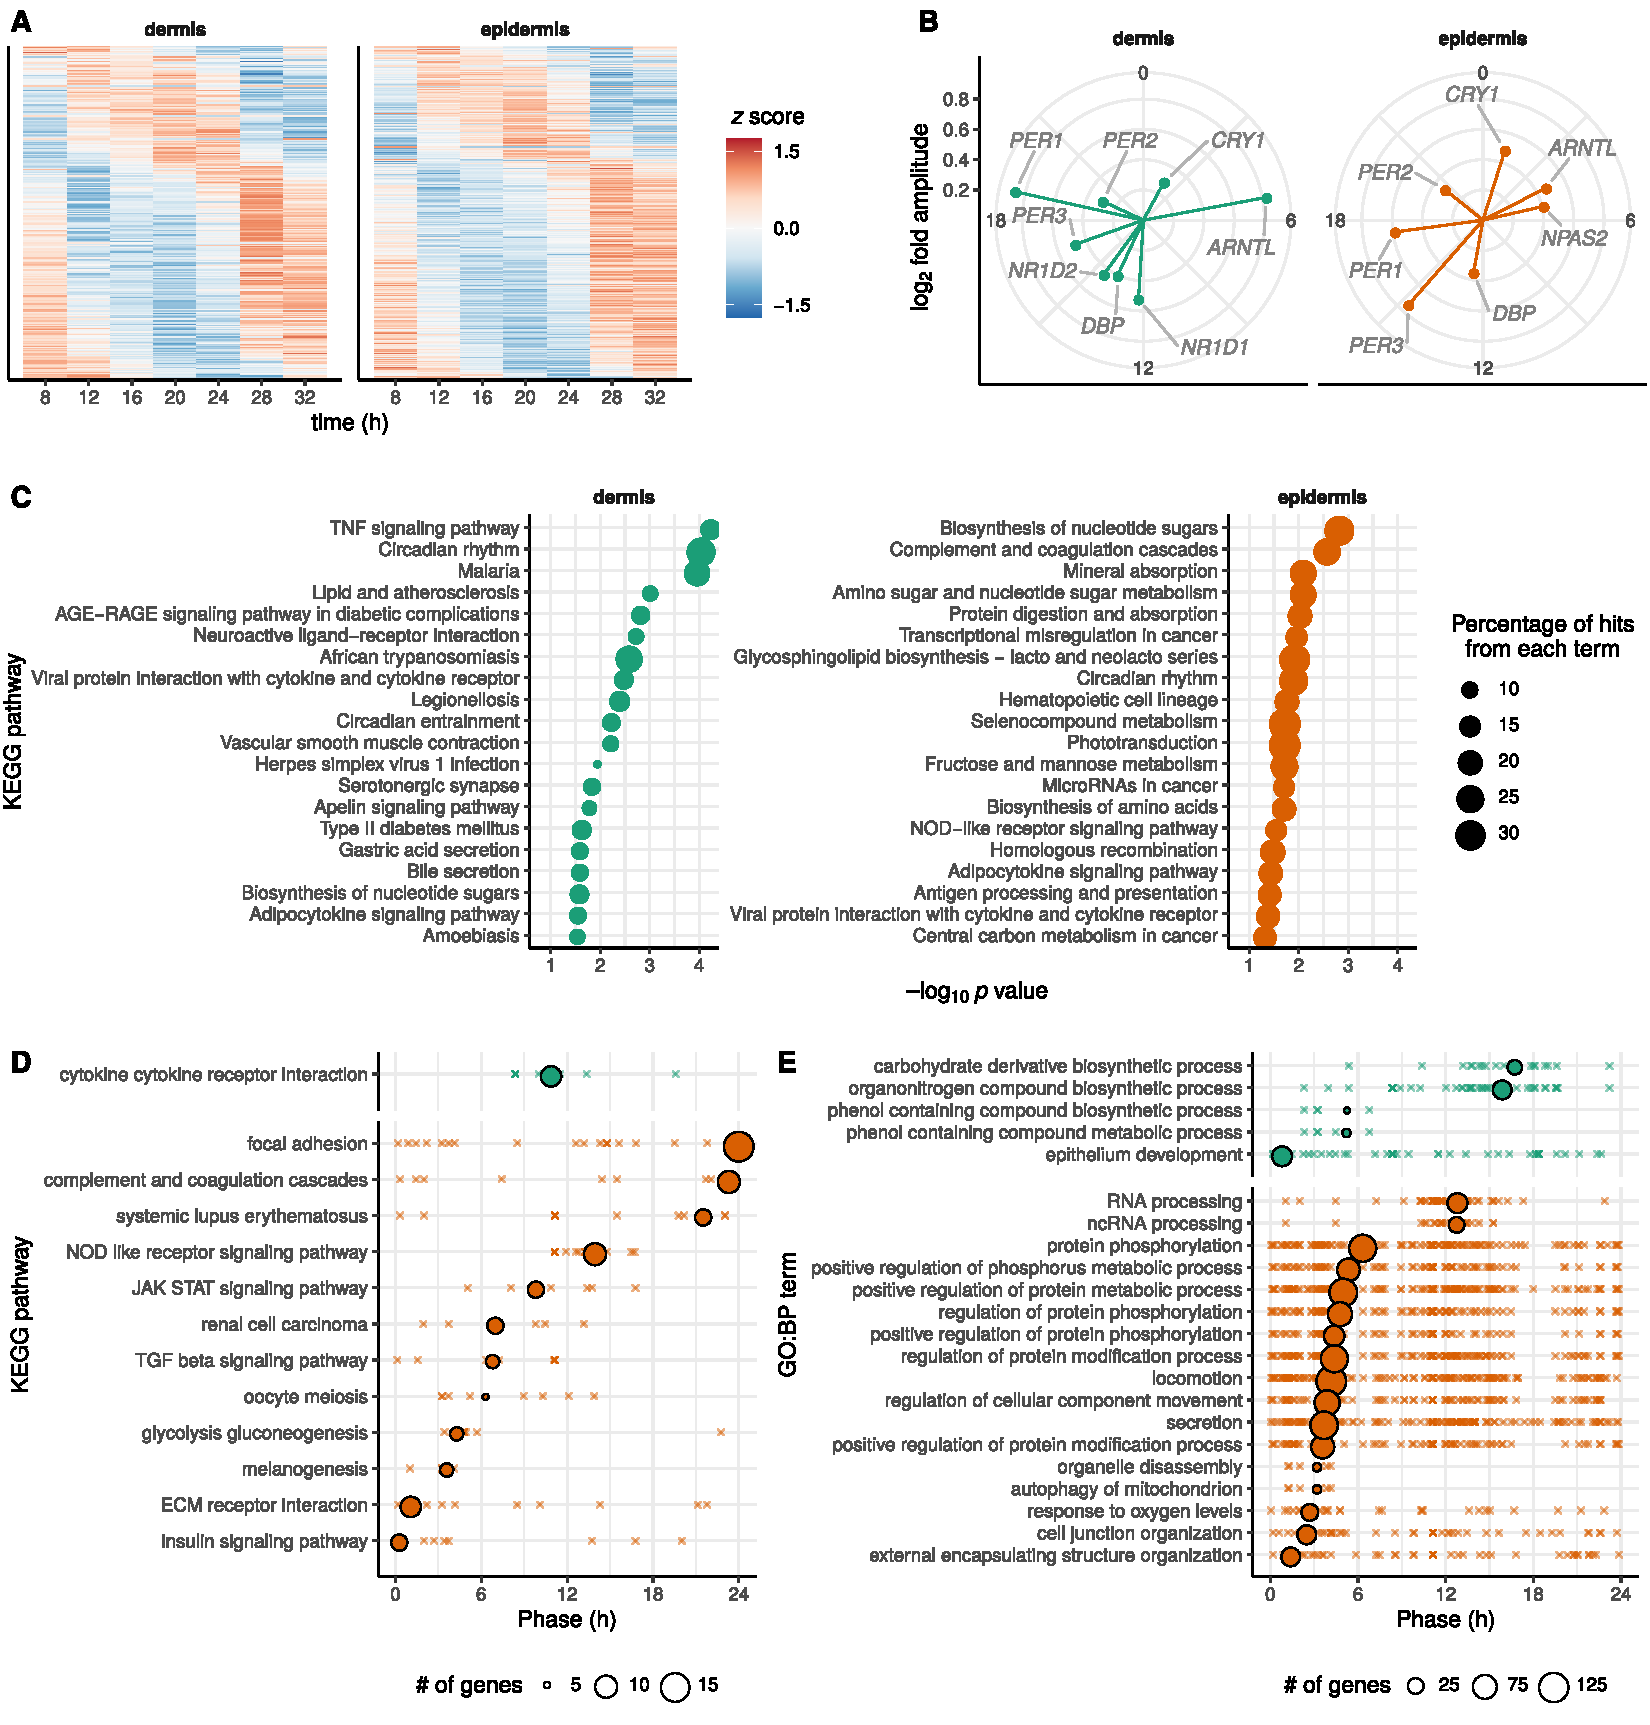
\includegraphics[scale=0.55]{./Figures/suppfig2.pdf}
		%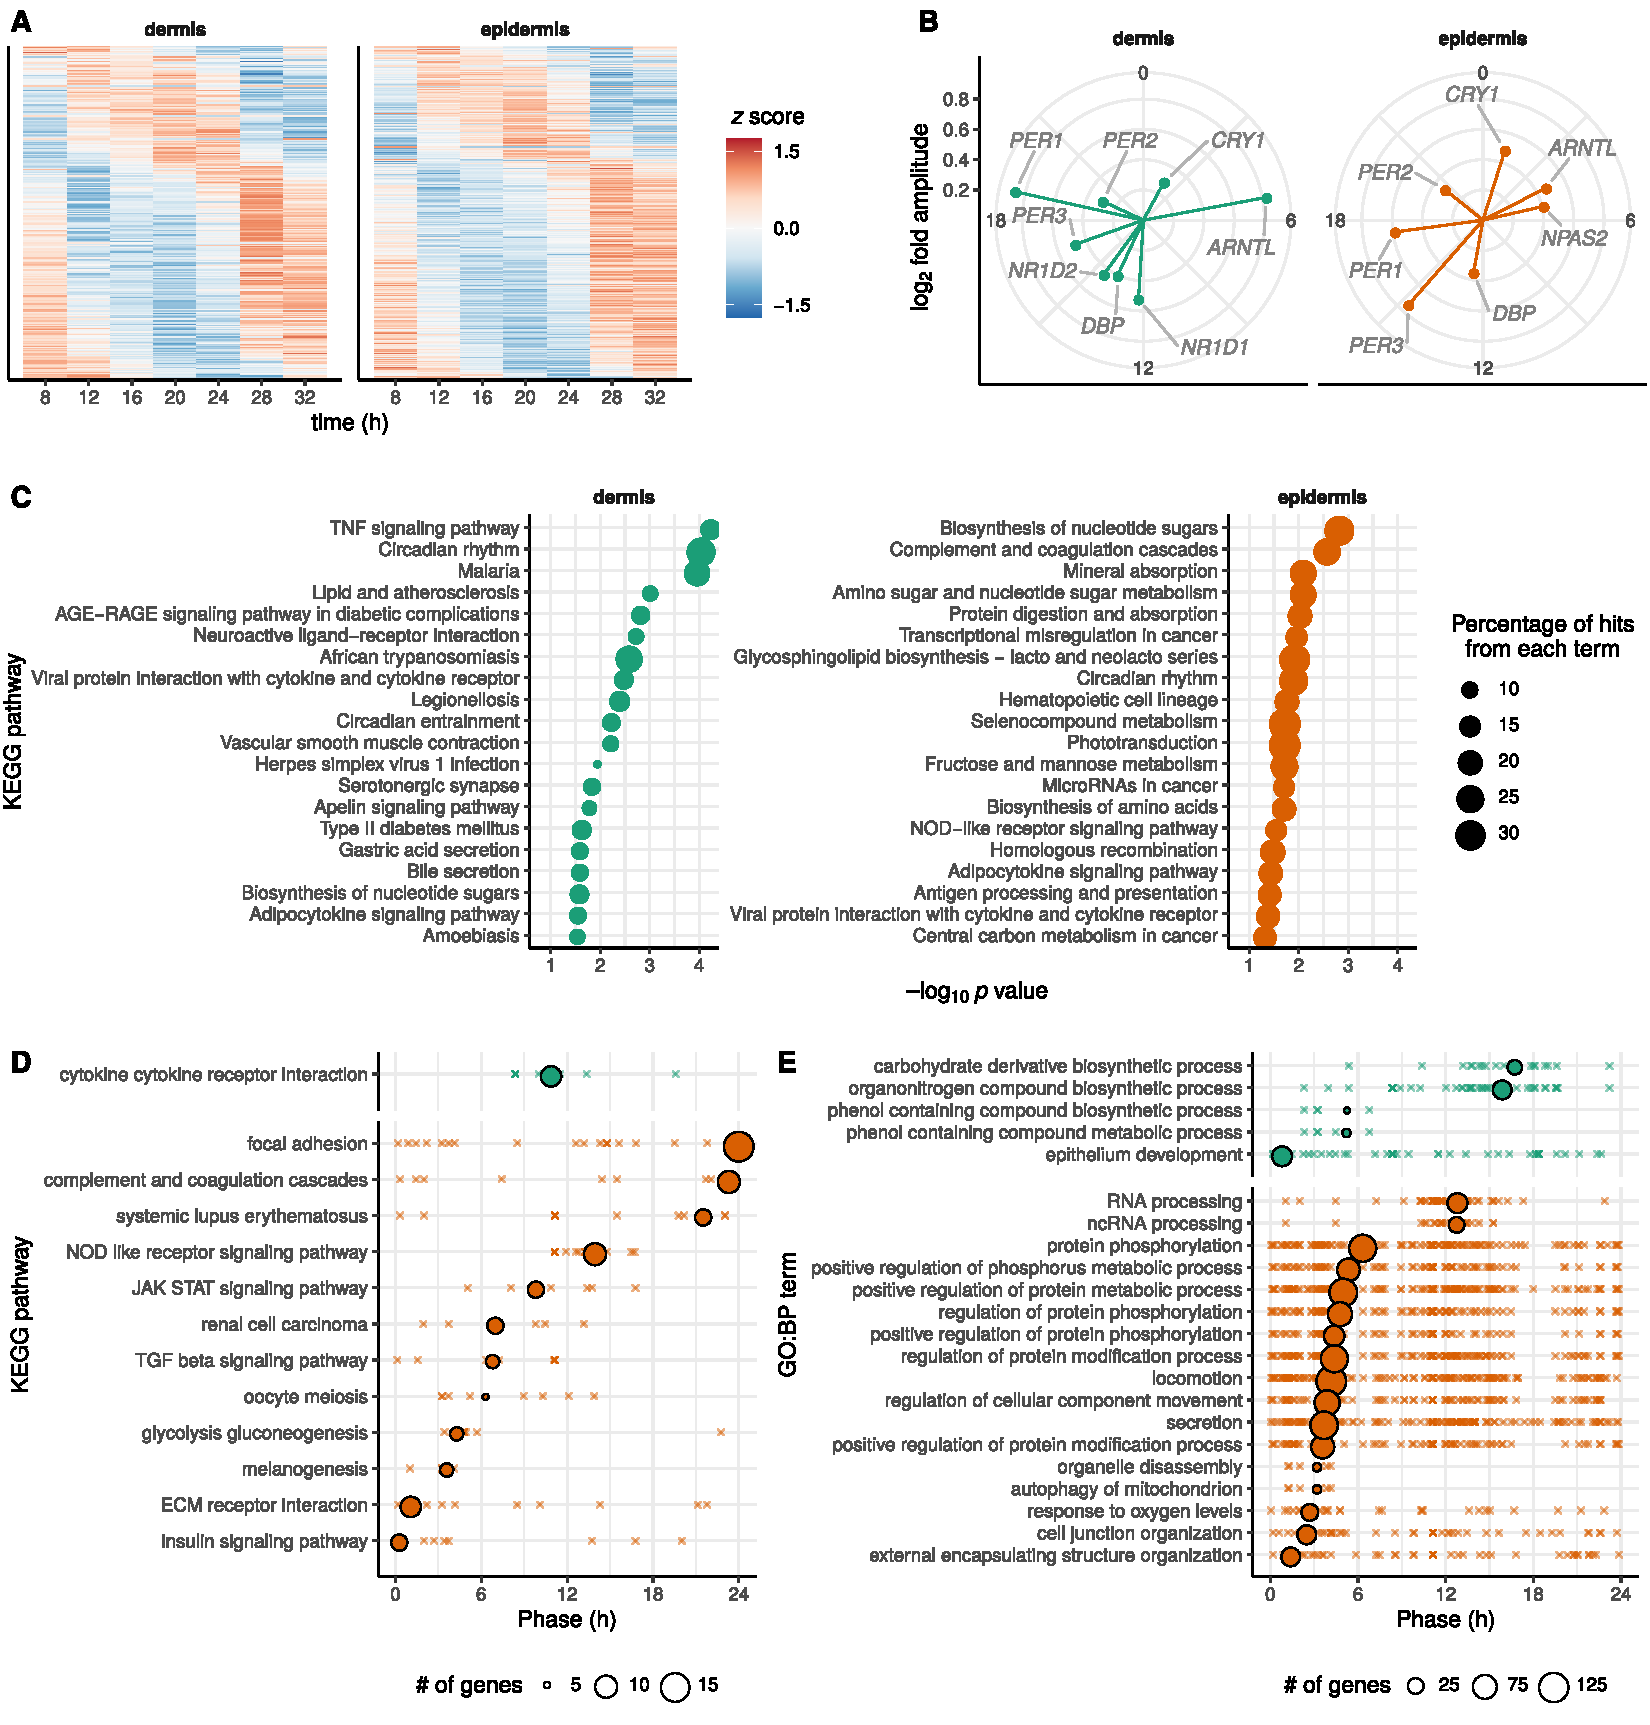
\includegraphics[scale=0.55]{./Figures/suppfig2.pdf}
		\caption{\textbf{Population circadian gene expression in healthy human skin.} \textbf{A.} $z$ score-normalized, acrophase-ordered expression heatmap of the circadian genes from human dermis (left) and epidermis (right).\textbf{ B.} Expression profiles of circadian core clock genes in human dermis (left) and epidermis (right). Arrow direction represents phase (expressed as peak time, in hours, after $\textrm{MSF}_\textrm{sc}$) and arrow length depicts peak-to-trough fold change amplitude. \textbf{C. }Circadian KEGG pathway enrichment analysis of the rhythmic genes in dermis (green) and epidermis (orange). The top 20 enriched pathways (with a minimum of 5 genes per category) in each layer are shown. \textbf{D.} Summary of significantly phase-clustered circadian GO terms ($q<0.05$) and KEGG pathways ($q<0.25$) in dermis (green) and epidermis (orange) as determined by PSEA (sets containing fewer than five circadian genes were excluded from the analysis). }%Heatmaps of Spearman correlation (rho) between each pair of core-clock genes for human dermis and epidermis. q < 0·01}
		\label{fig:suppfig2}
	\end{center}
\end{figure*}

%----------------------------------------------------------------------------------------
%----------------------------------------------------------------------------------------

\begin{figure*}[htb!]
	\begin{center}
		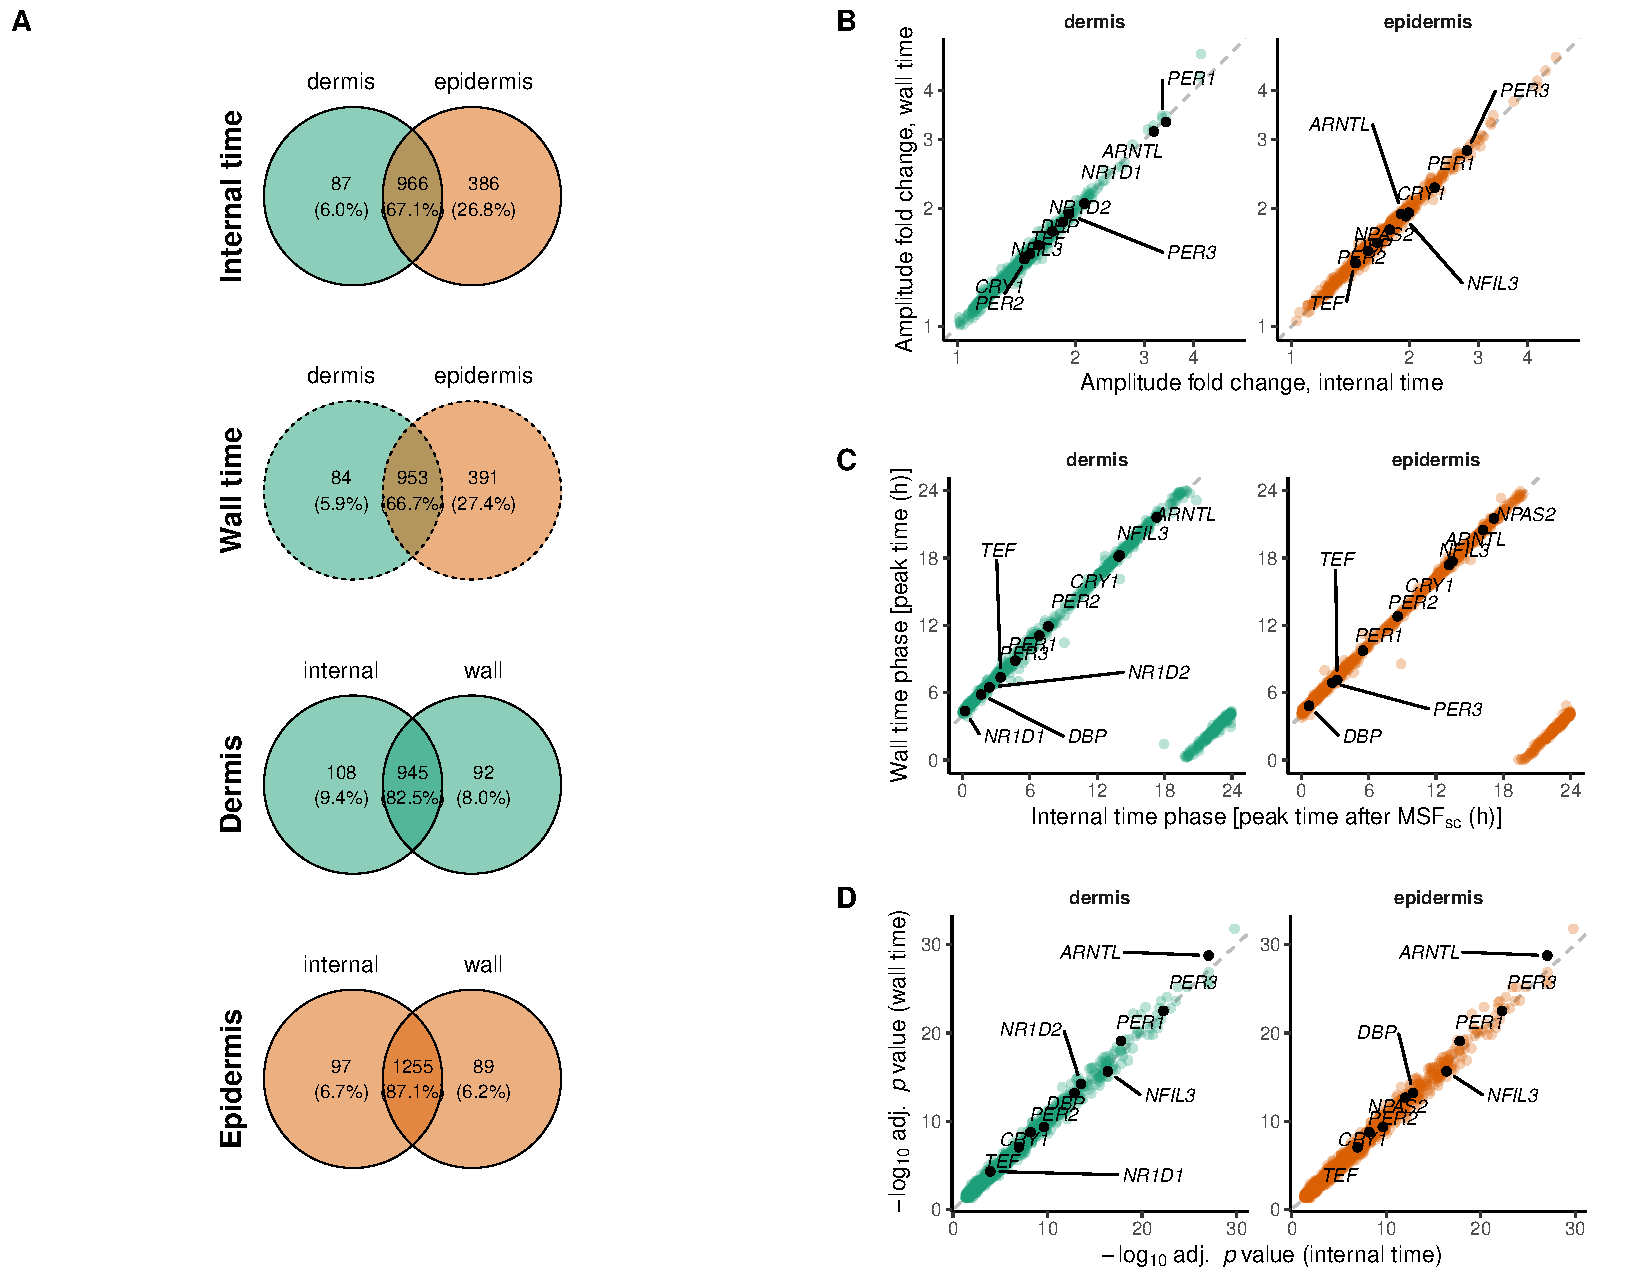
\includegraphics[scale=0.55]{./Figures/suppfig1.pdf}
		\caption{\textbf{Population circadian rhythms in human skin are similar when time is not adjusted for chronotype differences.} \textbf{A.} Venn diagram visualization of the number of genes identified as circadian in dermis (green) vs. epidermis (orange) and in the analysis using internal time (i.e., after correcting for chronotype differences, solid line) or wall time (dashed line). \textbf{B.} Amplitude correlation of genes identified as rhythmic with the internal time analysis compared to external time analysis. \textbf{C.} Phase correlation of circadian genes identified with the internal time analysis compared to external time analysis. Phase with respect to internal time was defined as peak time after $\textrm{MSF}_\textrm{sc}$, while phase with respect to wall time is the peaking time of the respective gene without correction. \textbf{D. }BH-adjusted \textit{p} value correlation of rhythmic genes identified with internal vs. external time analysis. \\
		% \textcolor{red}{Also to the question of whether genes with higher amplitude in internal time analysis are related to some specific functions, see noter on 9.9.21, nothing too interesting. inkscape: wall time in dashed}
	}
		\label{fig:suppfig1}
	\end{center}
\end{figure*}
\clearpage

%----------------------------------------------------------------------------------------
%----------------------------------------------------------------------------------------

%\begin{figure*}[h!tb]
%	\begin{center}
%		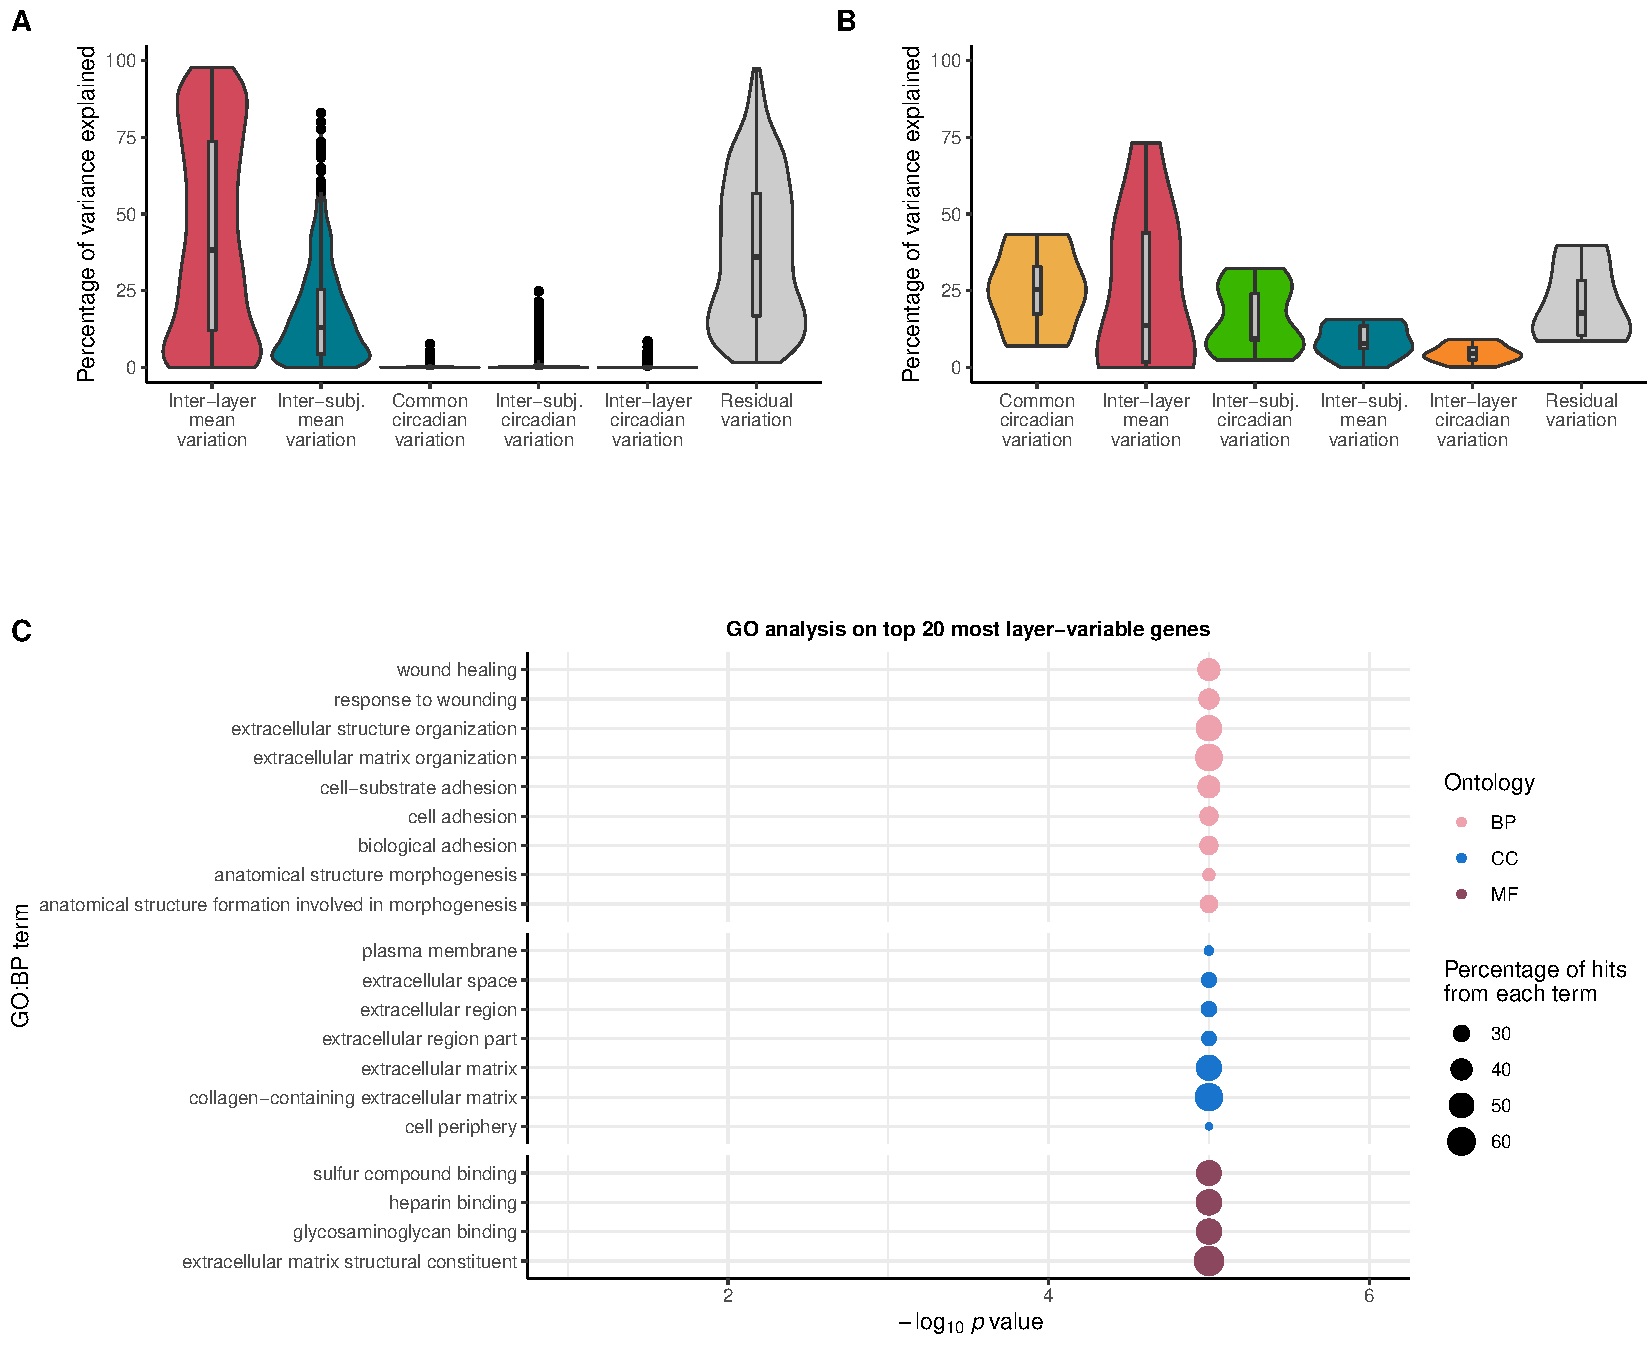
\includegraphics[scale=0.55]{./Figures/suppfig3_1.pdf}
%		\caption{\textbf{Drivers of variation in the human skin circadian transcriptome. A.} Negative control of the \texttt{variancePartition} analysis: the pipeline was run in 1000 non-rhythmic genes (FDR$>$0.1) to show that external time does not represent a major source of variation among these transcripts. \textbf{B.} Positive control: \texttt{variancePartition} was run in the clock genes to show that time represents a major (in fact, the largest) source of variation.\textbf{ C.} GO enrichment analysis in the 200 circadian transcripts with largest variability in mean expression across layers. \textbf{D.} GO enrichment analysis in the 200 rhythmic transcripts with largest rhythm variability across layers, i.e., transcripts that show differential rhythms in human dermis versus epidermis. \textbf{E.} GO enrichment analysis in the 200 circadian transcripts with largest residual variability in mean expression. For C-E: the top 20 enriched terms (with a minimum gene set of 5 terms from each category) are shown; pink represents biological processes; blue, cellular compartment; purple, molecular function; enrichment was performed testing against the background of $\sim$1400 rhythmic genes in at least one layer.} %	Variance partition with external time. Positive and negative control + go analysis of top 200 most changing genes from categories of interest. background of go analyses are all rhythmic genes in D or E. GO with clusterProfiler, mingene set size=5}
%		\label{fig:suppfig3}
%	\end{center}
%\end{figure*}
%\clearpage
%
%\begin{figure*}[h!tb]
%	\begin{center}
%		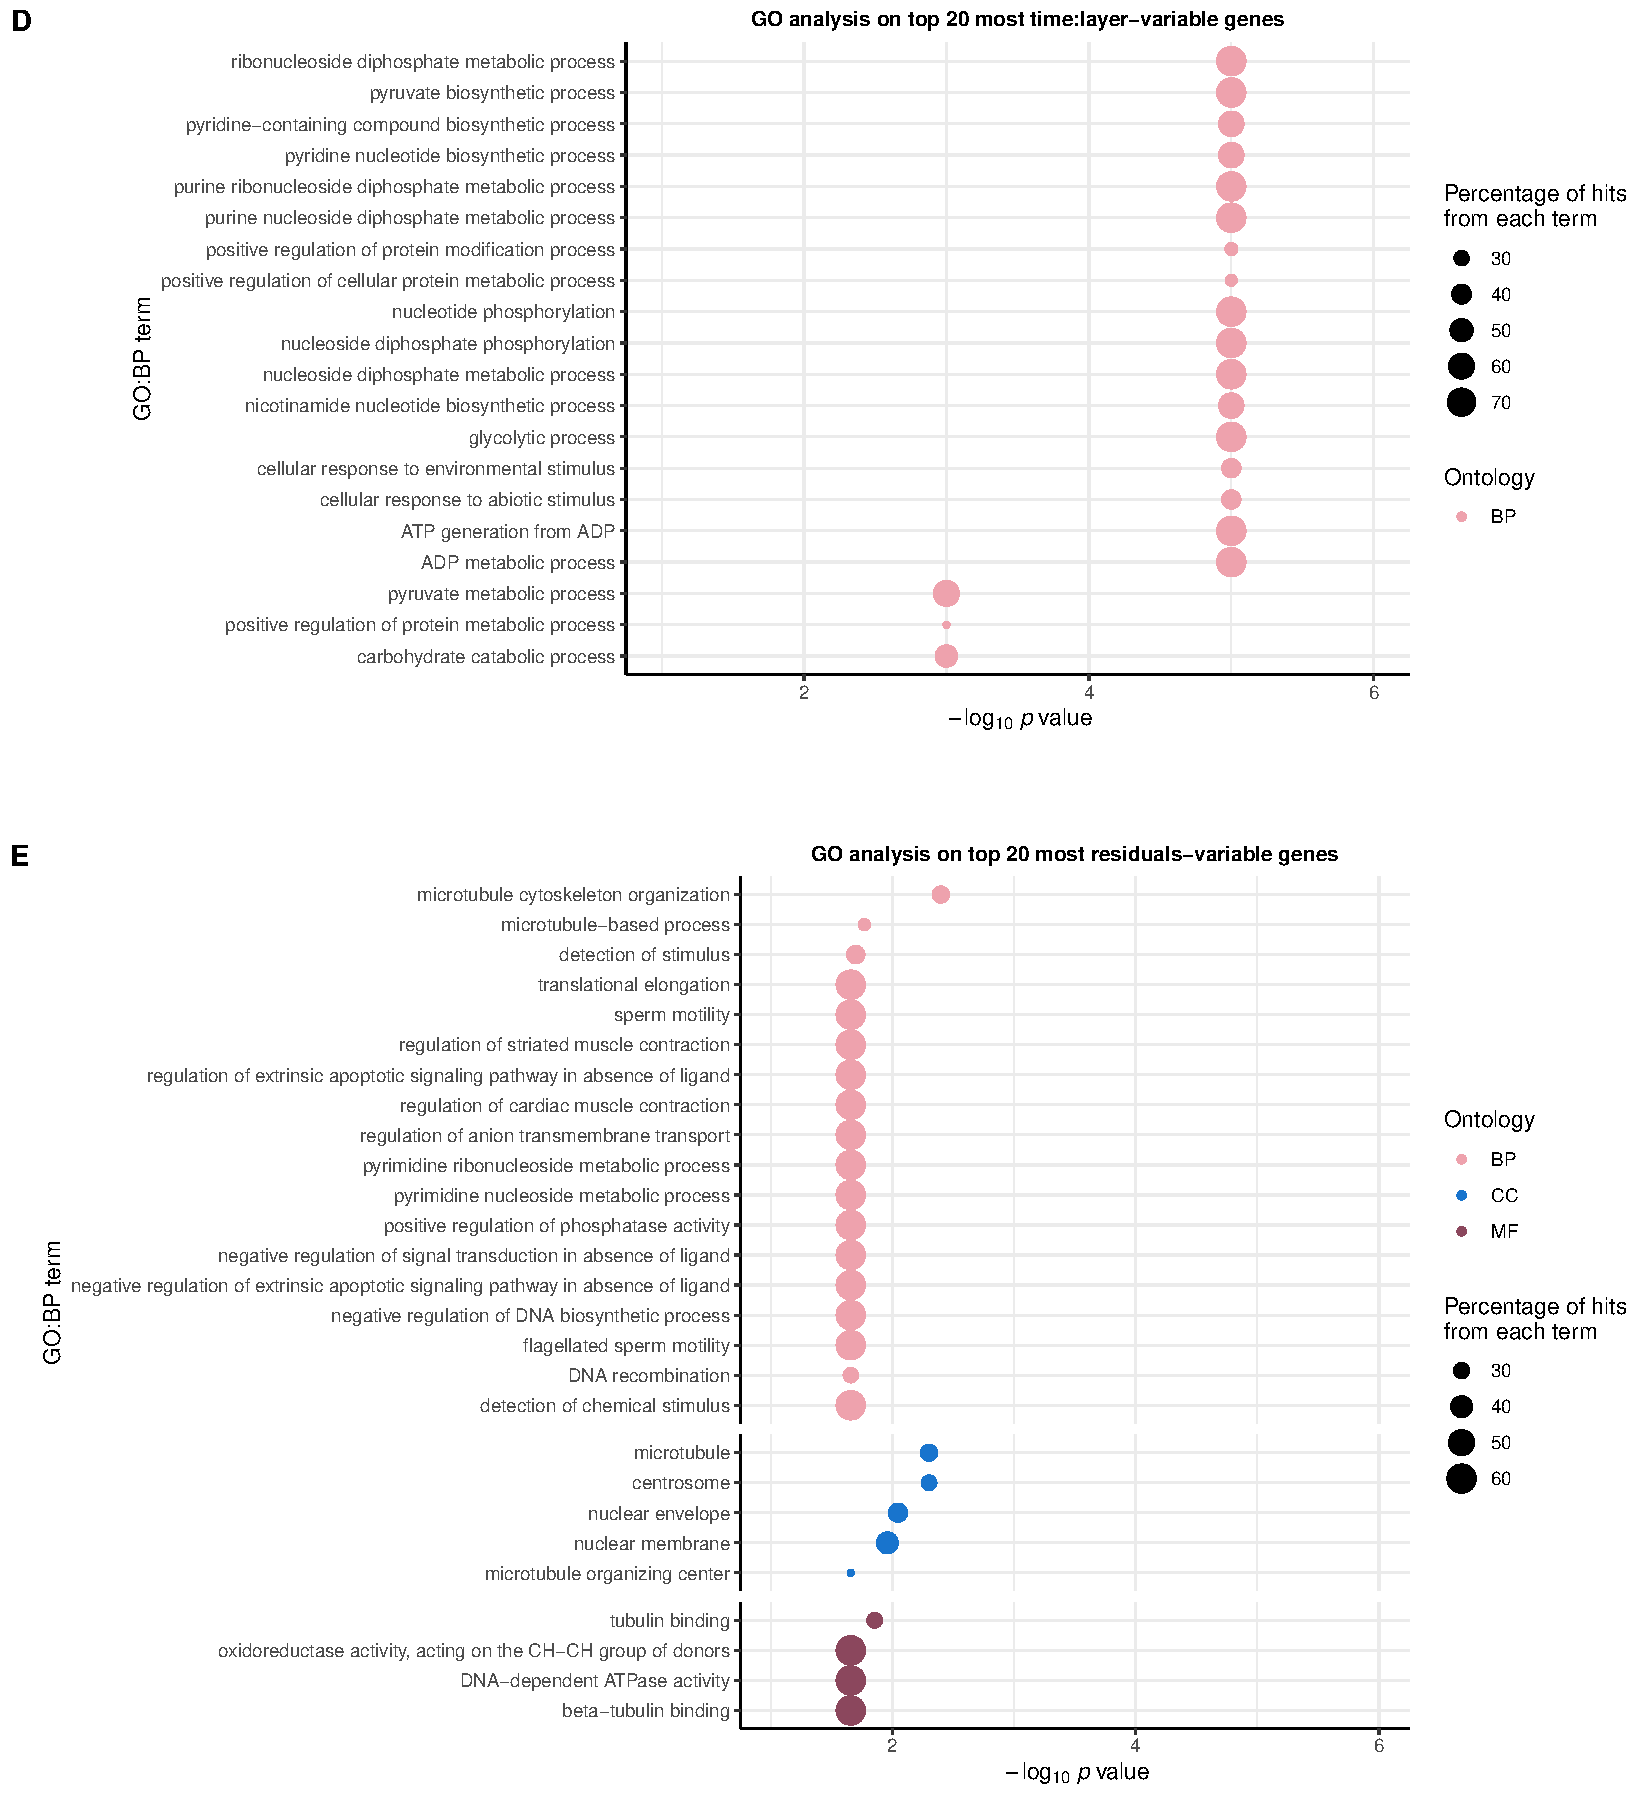
\includegraphics[scale=0.55]{./Figures/suppfig3_2.pdf}
%		%\caption*{Suppfig3 continuation}
%		%\label{fig:suppfig2}
%	\end{center}
%\end{figure*}
\clearpage


%----------------------------------------------------------------------------------------
%----------------------------------------------------------------------------------------

%\begin{figure*}[h!tb]
%	\begin{center}
%		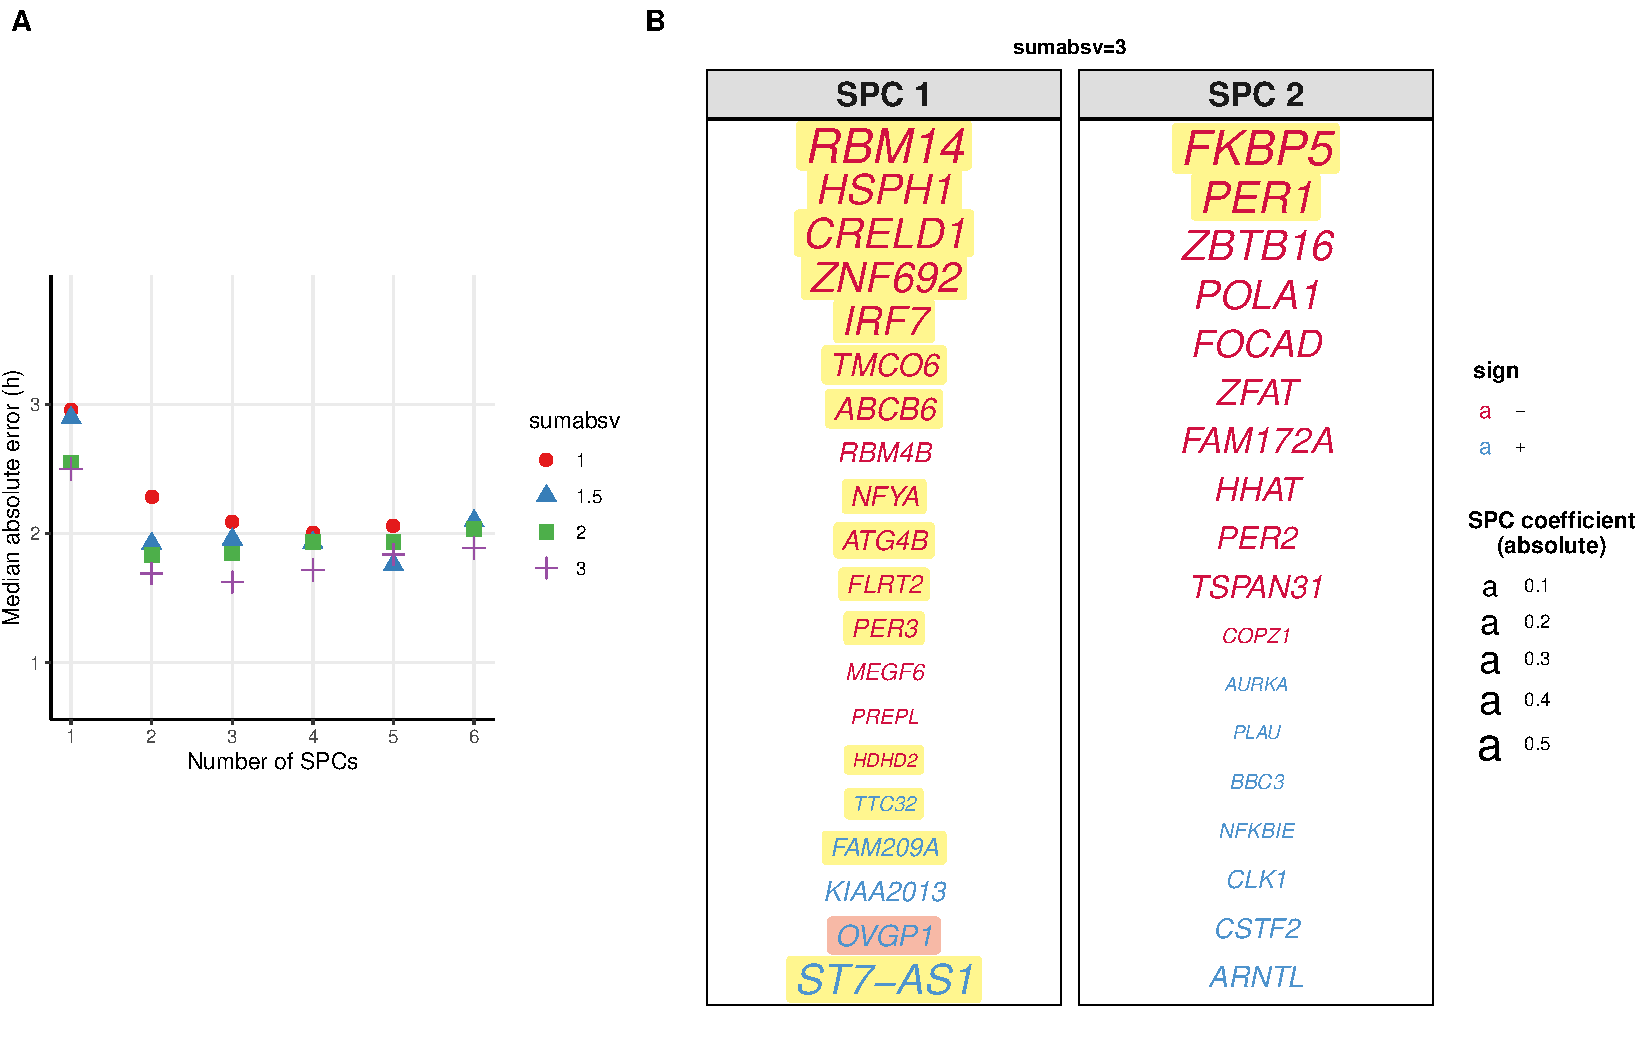
\includegraphics[scale=0.55]{./Figures/suppfig4.pdf}
%		\caption{\textbf{Identification of internal time-telling genes in human skin with \texttt{ZeitZeiger} \cite{Hughey2016}. A.} Median absolute error of the internal-time prediction on cross-validation (see Materials and Methods for details) as a function of the two main parameters of \texttt{ZeitZeiger}, \texttt{sumabsv} and \texttt{nSPC}. \textbf{B. }Internal time predictors from human skin for \texttt{sumabsv}=3 and \texttt{nSPC}=2. Genes assigned to SPC1 or SPC2 as well as their coefficients are shown. Highlighted in yellow are genes that appeared in the top 20 most common circadian varying genes in the \texttt{variancePartition }analysis done in the rhythmic genes in human skin (i.e., in \textit{at least} one layer); in orange, genes that showed differential rhythms across layers (i.e., genes with high inter-layer circadian variation from the \texttt{variancePartition} analysis). Note, that the difference to Figure \ref{fig:fig3} is that here, \texttt{ZeitZeiger} was run once using the whole $\sim$11000 expressed genes in at least one layer, and not separately in each layer.}%ZeitZeiger with internal time in skin as a whole -- worse MAE
%		\label{fig:suppfig4}
%	\end{center}
%\end{figure*}
\clearpage

%----------------------------------------------------------------------------------------
%----------------------------------------------------------------------------------------

\begin{figure*}[h!tb]
	\begin{center}
		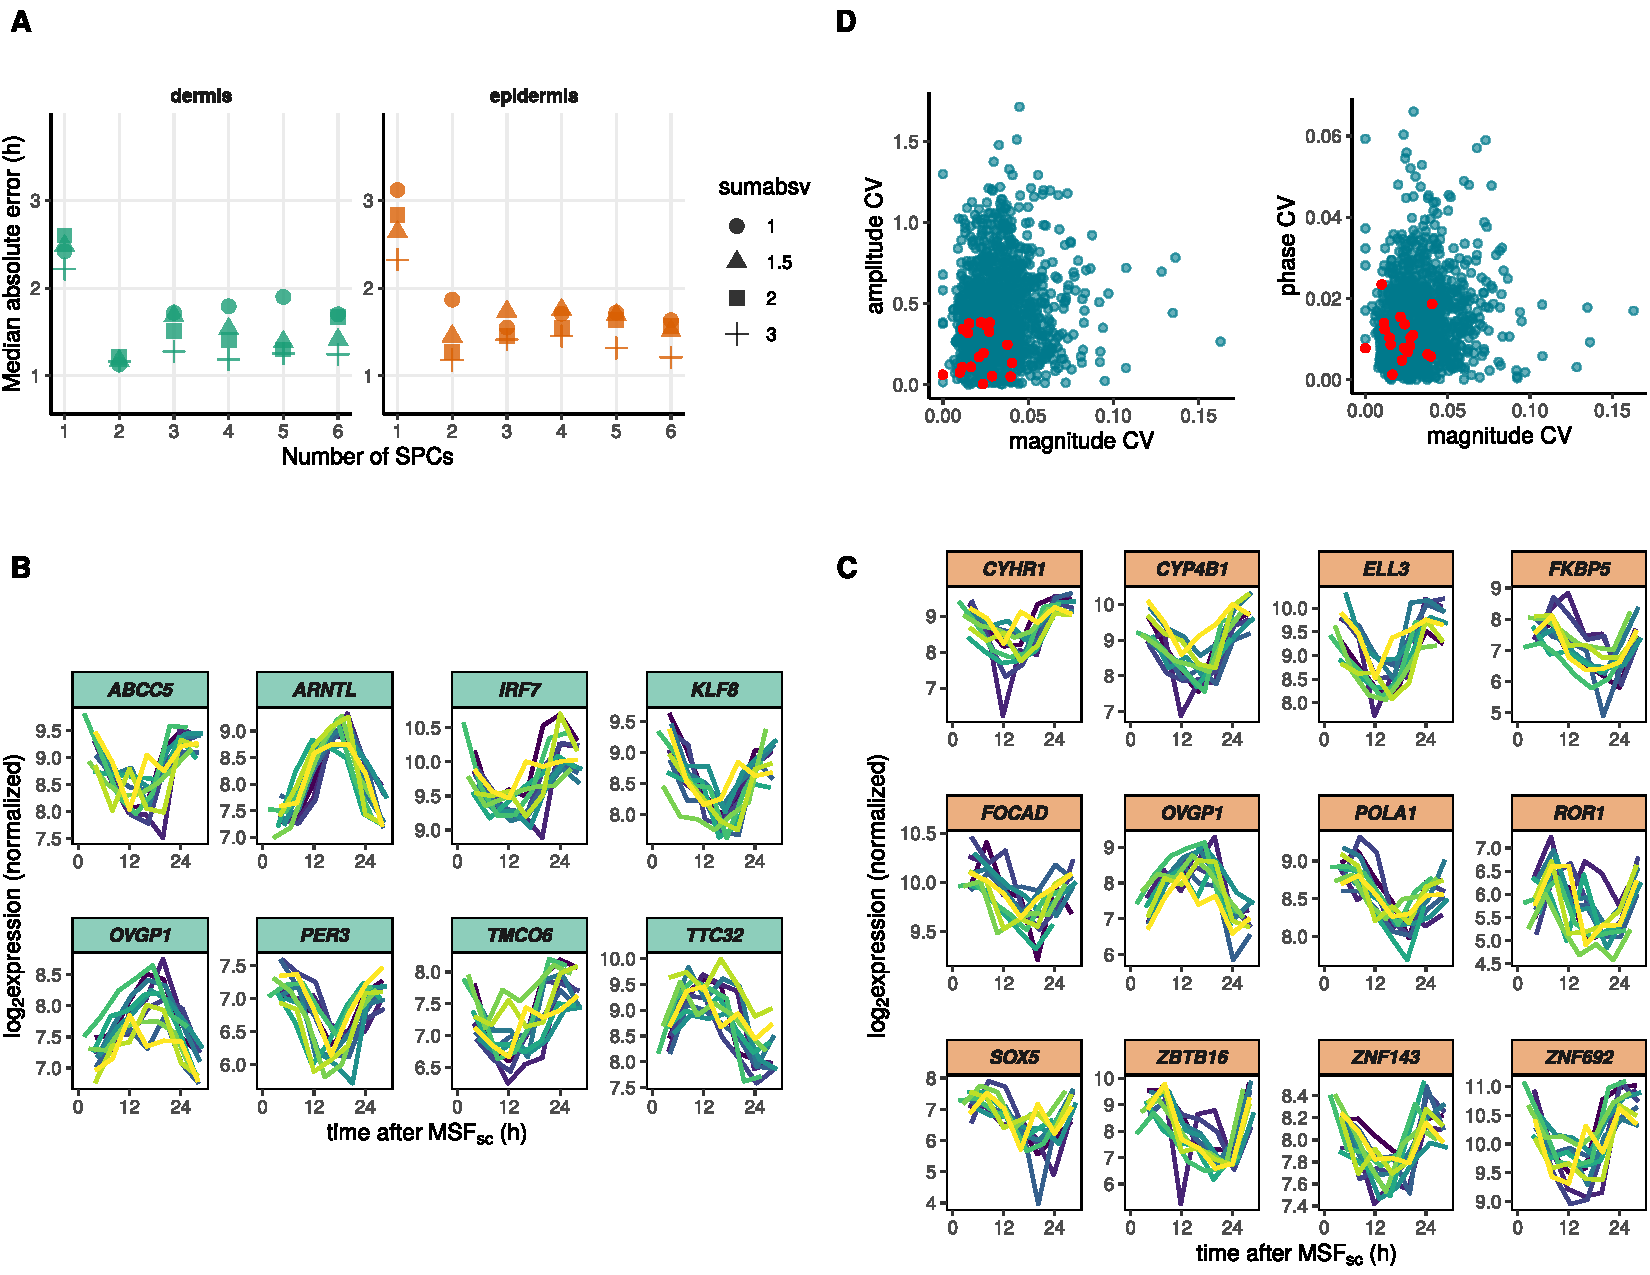
\includegraphics[width=\textwidth]{./Figures/suppfig5.pdf}
		\caption{\textbf{Predictive biomarkers of internal time in human dermis and epidermis. A. }Median absolute error of the internal-time prediction on cross-validation (see Materials and Methods for details) as a function of the two main parameters of \texttt{ZeitZeiger}, \texttt{sumabsv} and \texttt{nSPC}. \textbf{B.} Quantification of magnitude, amplitude and phase variability of circadian genes across subjects. Predictive biomarkers are shown in red. \textbf{C.} Expression profiles of the time-telling genes in dermis (green) and \textbf{D.} epidermis (orange) for optimal parameter choice of \texttt{sumabsv} and \texttt{nSPC}. Colored lines represent the time series in different subjects. \texttt{ZeitZeiger} was run with all $\sim11000$ expressed genes, separately for dermis and epidermis.}%ZeitZeiger in D and E separately with internal time. A) Timeseries of dermal ZZ genes
		%\textbf{D.} Expression profiles of the time-telling genes from our cohort in dermis (left) and epidermis (right) represented in SPC space and faceted by subject. Colors indicate internal time. 
		\label{fig:suppfig5}
	\end{center}
\end{figure*}
\clearpage

%\begin{figure*}[h!tb]
%	\begin{center}
%		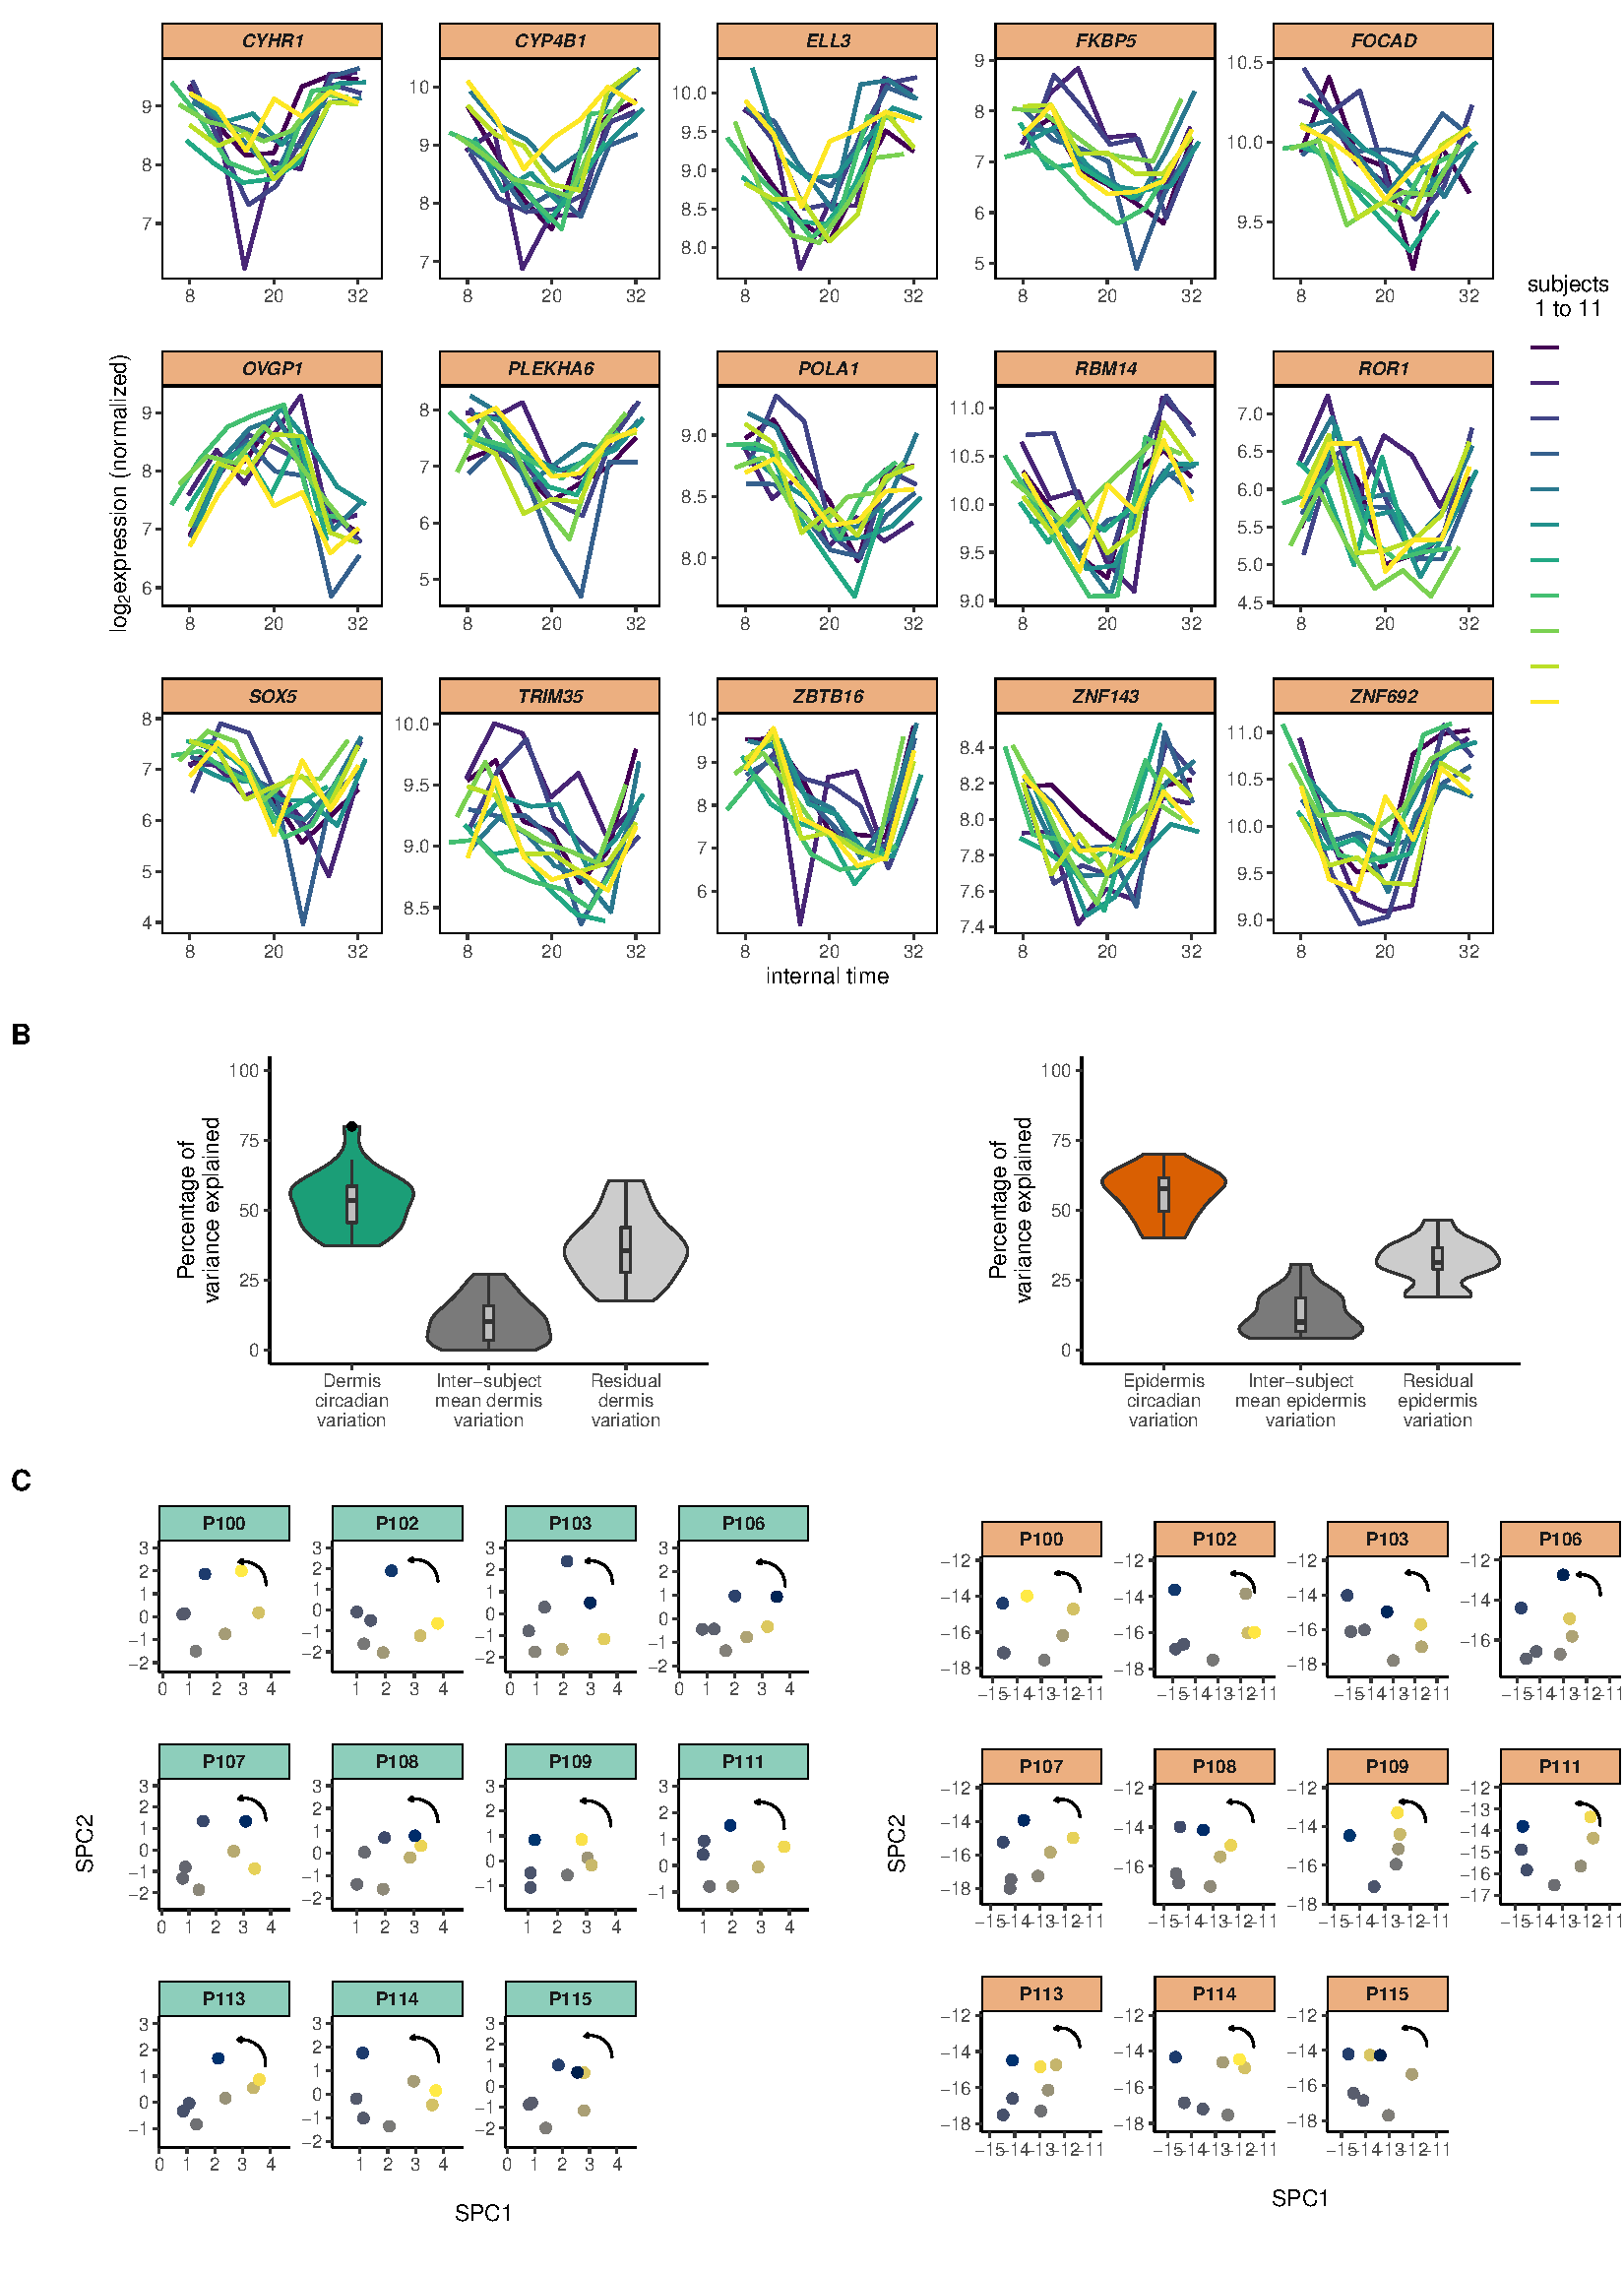
\includegraphics[scale=0.55]{./Figures/suppfig5_2.pdf}
%		%\caption*{Continuation of Suppfig5. ZeitZeiger in D and E separately with internal time. A) Timeseries of epidermal ZZ genes}
%		%\label{fig:suppfig2}
%	\end{center}
%\end{figure*}
\clearpage


%----------------------------------------------------------------------------------------
%----------------------------------------------------------------------------------------

\begin{table}[h!tb]\vspace{-.4cm}
	\caption{\textbf{Information and sleeping schedules of the healthy subjects who participated in the study.} Chronotypes were estimated from sleep schedules as the mid-sleep time on free days after correcting for sleep debt ($\textrm{MSF}_\textrm{sc}$) \cite{Roenneberg2007, Vetter2021}.}
	\footnotesize \vspace{-.2cm}
	\begin{tabular}{ccccccccc}
		\hline
		\textbf{Subject} &
		\textbf{Sex} &
		\textbf{\begin{tabular}[c]{@{}c@{}}Birth\\year\end{tabular}} &
		\textbf{\begin{tabular}[c]{@{}c@{}}Bed time\\work days\end{tabular}} &
		\textbf{\begin{tabular}[c]{@{}c@{}}Sleep time\\work days\end{tabular}} &
		\textbf{\begin{tabular}[c]{@{}c@{}}Min\\fall asleep\\work days\end{tabular}} &
		\textbf{\begin{tabular}[c]{@{}c@{}}Wake up time\\work days\end{tabular}} &
		\textbf{\begin{tabular}[c]{@{}c@{}}Min\\wake up\\work days\end{tabular}} &
		\textbf{\begin{tabular}[c]{@{}c@{}}Alarm\\work days?\end{tabular}} \\ \hline
		P108 & male   & 1984 & 22:45 & 23:00 & 20  & 6:30 & 15 & Y  \\ 
		P100 & male   & 1991 & 23:00 & 23:00 & 7.5 & 7:00 & 5  & Y  \\
		P113 & male   & 1985 & 23:30 & 0:00  & 30  & 8:30 & 10 & Y  \\ 
		P106 & male   & 1982 & 23:00 & 23:15 & 15  & 6:52 & 7.5& Y  \\ 
		P102 & male   & 1989 & 23:00 & 23:00 & 10  & 7:30 & 0  & Y  \\ 
		P109 & male   & 1984 & 23:00 & 23:00 & 5   & 8:00 & 0  & Y  \\ 
		P103 & female & 1988 & 0:00  & 0:25  & 25  & 7:30 & 9  & Y  \\ 
		P107 & female & 1987 & 23:00 & 23:00 & 15  & 6:00 & 5  & Y  \\ 
		P111 & female & 1983 & 0:00  & 0:00  & 5   & 8:00 & 15 & Y  \\ 
		P114 & female & 1986 & 23:30 & 23:30 & 5   & 8:30 & 5  & Y  \\ 
		P115 & female & 1981 & 22:00 & 22:15 & 5   & 5:20 & 5  & Y  \\ \hline
	\end{tabular}\vspace{0.2cm}
	\begin{tabular}{cccccccc}
		\hline
		\textbf{Subject} &
		\textbf{\begin{tabular}[c]{@{}c@{}}Wake up\\before alarm?\end{tabular}} &
		\textbf{\begin{tabular}[c]{@{}c@{}}Bed time\\free days\end{tabular}} &
		\textbf{\begin{tabular}[c]{@{}c@{}}Sleep time\\free days\end{tabular}} &
		\textbf{\begin{tabular}[c]{@{}c@{}}Min\\fall asleep\\free days\end{tabular}} &
		\textbf{\begin{tabular}[c]{@{}c@{}}Wake up time\\free days\end{tabular}} &
		\textbf{\begin{tabular}[c]{@{}c@{}}Wake up time\\free days\end{tabular}} &
		\textbf{\begin{tabular}[c]{@{}c@{}}Alarm\\free days?\end{tabular}} \\ \hline
		P108 & Y & 23:00 & 23:15 & 15 & 6:30  & 30 & N \\ 
		P100 & N & 0:00  & 0:00  & 5  & 8:00  & 15 & Y \\
		P113 & N & 1:00  & 1:15  & 20 & 9:30  & 15 & Y \\ 
		P106 & Y & 23:30 & 23:45 & 15 & 9:15  & 60 & Y \\ 
		P102 & N & 0:00  & 0:00  & 10 & 8:00  & 10 & N \\ 
		P109 & Y & 0:00  & 0:00  & 5  & 8:30  & 30 & N \\ 
		P103 & N & 0:00  & 0:00  & 25 & 7:30  & 5  & Y \\ 
		P107 & Y & 0:00  & 0:00  & 15 & 7:30  & 5  & N \\ 
		P111 & Y & 2:30  & 2:30  & 5  & 11:00 & 30 & N \\ 
		P114 &   & 23:30 & 23:30 & 5  & 8:30  & 5  & N \\ 
		P115 & N & 0:00  & 0:15  & 5  & 8:30  & 30 & N \\ \hline
	\end{tabular}\vspace{0.2cm}
	\begin{tabular}{cc}
		\hline
		\textbf{Subject} & \textbf{\begin{tabular}[c]{@{}c@{}}Corrected\\mid sleep time\end{tabular}} \\ \hline
		P108             & 02:58           \\
		P100             & 04:00           \\
		P113             & 05:28           \\
		P106             & 03:50           \\
		P102             & 04:11           \\
		P109             & 04:26           \\
		P103             & 03:36           \\
		P107             & 03:34           \\
		P111             & 06:34           \\
		P114             & 04:00           \\
		P115             & 03:58          \\ \hline
	\end{tabular}	
	\label{tab:supptab1}
\end{table}

%----------------------------------------------------------------------------------------
%----------------------------------------------------------------------------------------

%https://genomemedicine.biomedcentral.com/articles/10.1186/s13073-020-00768-9#Sec19
%\begin{table}[b!ht]\vspace{-.3cm}
%	\caption{\textbf{List of software packages used in this study.} Versions and references are included. }\vspace{-.2cm}
%	\footnotesize
%	\centering
%\begin{tabular}{llc}
%	\hline
%	\textbf{\begin{tabular}[c]{@{}c@{}}Software\\package\end{tabular}} & \textbf{Version} & \textbf{Ref.}     \\ \hline
%	Biobase                   & 2.46.0           & \cite{biobase}         \\
%	clusterProfiler           & 3.14.3           & \cite{clusterprofiler} \\
%	cowplot                   & 1.1.1            & \cite{cowplot}         \\
%	doParallel                & 1.0.16           & \cite{doparallel}      \\
%	dplyr                     & 1.0.5            & \cite{dplyr}           \\
%	GEOquery                  & 2.54.1           & \cite{geoquery}        \\
%	ggforce                   & 0.3.3            & \cite{ggforce}         \\
%	ggplot2                   & 3.3.3            & \cite{ggplot2}         \\
%	ggrepel                   & 0.9.1            & \cite{ggrepel}         \\
%	ggthemes                  & 4.2.4            & \cite{ggthemes}        \\ \hline
%\end{tabular}	
%\hspace{0.2cm}
%\begin{tabular}{llc}
%	\hline
%	\textbf{\begin{tabular}[c]{@{}c@{}}Software\\package\end{tabular}} & \textbf{Version} & \textbf{Ref.}     \\ \hline
%	ggvenn                    & 0.1.8            & \cite{ggvenn}          \\
%	hgug4112a.db              & 3.2.3            & \cite{hgug4112a}       \\
%	hms                       & 1.0.0            & \cite{hms}             \\
%	limma                     & 3.42.2           & \cite{limma}           \\
%	lubridate                 & 1.7.10           & \cite{lubridate}       \\
%	magrittr                  & 2.0.1            & \cite{magrittr}        \\
%	msigdbr                   & 7.4.1            & \cite{msigdbr}         \\
%	\textcolor{red}{oligo??}  &                  & \textbf{which?}        \\
%	PSEA                      & 1.1              & \cite{Zhang2016}       \\
%	R                         & 3.6.3            & \cite{R}               \\ \hline
%\end{tabular}
%\hspace{0.2cm}	
%\begin{tabular}{llc}
%	\hline
%	\textbf{\begin{tabular}[c]{@{}c@{}}Software\\package\end{tabular}} & \textbf{Version} & \textbf{Ref.}     \\ \hline
%	stringr                   & 1.4.0            & \cite{stringr}         \\
%	tibble                    & 3.1.1            & \cite{tibble}          \\
%	tidyr                     & 1.1.3            & \cite{tidyr}           \\
%	tidytext                  & 0.3.2            & \cite{tidytext}        \\
%	tidyverse                 & 1.3.1            & \cite{tidyverse}       \\
%	variancePartition         & 1.16.1           & \cite{Hoffman2016}     \\
%	viridis                   & 0.6.1            & \cite{viridis}         \\
%	zeitzeiger                & 2.0.2            & \cite{Hughey2016}      \\ 
%	                          &                  &                        \\
%	                          &                  &                        \\ \hline
%\end{tabular}	
%	\label{tab:supptab2}

%\end{table}
\clearpage

\beginsupplement

%----------------------------------------------------------------------------------------
%	REFERENCE LIST
%----------------------------------------------------------------------------------------
\newpage
\footnotesize
\bibliography{References}
\bibliographystyle{naturemag}
%------------------------------------------------

\end{document}

